\selectlanguage{english}

\section{Metric manifolds}

\begin{definition}
  A \textit{metric} $ g $ is a (0,2) tensor field on a manifold $ \mathcal{M} $ that is:
  \begin{enumerate}
    \item symmetric: $ g(X,Y) = g(Y,X) $;
    \item non-degenerate: $ \exists p \in \mathcal{M} : g(X,Y)\vert_p = 0 \,\forall Y \in T_p \mathcal{M} \,\Rightarrow\, X_p = 0 $.
  \end{enumerate}
\end{definition}

\begin{definition}
  A \textit{metric manifold} $ (\mathcal{M},g) $ is a manifold equipped with a metric.
\end{definition}

With a choice of coordinates, the metric can be written as:
\begin{equation}
  g = g_{\mu \nu}(x) dx^{\mu} \otimes dx^{\nu}
  \label{eq:3.1}
\end{equation}
where:
\begin{equation}
  g_{\mu \nu} = g\left( \frac{\pa}{\pa x^{\mu}}, \frac{\pa}{\pa x^{\nu}} \right)
  \label{eq:3.2}
\end{equation}
It is often written also as $ ds^2 = g_{\mu \nu}(x) dx^{\mu} dx^{\nu} $. The matrix $ g_{\mu \nu}(x) \in \R^{n \times n} $ is symmetric, and there's always a choice of basis on each tangent space such that this matrix is diagonal: the non-degeneracy condition implies that none of the diagonal elements vanish.

\begin{proposition}
  The \textit{signature} of a metric, i.e. the number of negative entries when diagonalized, is independent on the choice of basis.
\end{proposition}
\begin{proof}
  From Sylvester's theorem of inertia.
\end{proof}

\paragraph{Riemannian manifolds}

\begin{definition}
  A \textit{Riemannian manifold} $ (\mathcal{M},g) $ is a manifold equipped with a metric with totally-positive signature.
\end{definition}

\begin{example}
  The Euclidean space $ \R^n $, equipped with the metric $ g_{\mu \nu} = \delta_{\mu \nu} $ (in Cartesian coordinates), is a Riemannian manifold.
\end{example}

\begin{definition}
  Given a Riemannian manifold $ (\mathcal{M},g) $ and $ X \in \xm $, the \textit{length} of $ X $ at $ p \in \mathcal{M} $ is:
  \begin{equation}
    \abs{X_p} \defeq \sqrt{g(X,X)\vert_p}
    \label{eq:3.3}
  \end{equation}
  Given $ Y \in \xm $, the \textit{angle} between $ X $ and $ Y $ at $ p \in \mathcal{M} $ is:
  \begin{equation}
    \cos \theta \defeq \frac{g(X,Y) \vert_p}{\abs{X_p} \abs{Y_p}}
    \label{eq:3.4}
  \end{equation}
\end{definition}

This can be generalized to distances between points on a curve $ \sigma : \mathcal{\R} \rightarrow \mathcal{M} $:
\begin{equation}
  d(p,q) = \int_a^b dt \sqrt{g(X,X)\vert_{\sigma(t)}}
  \label{eq:3.5}
\end{equation}
where $ \sigma(a) = p $, $ \sigma(b) = q $ and $ X $ is the tangent vector field of the curve. With parametrization $ x^{\mu}(t) $, the tangent vector has components $ X^{\mu} = \frac{dx^{\mu}}{dt} $, thus:
\begin{equation}
  d(p,q) = \int_a^b dt \sqrt{g_{\mu \nu}(x) \frac{dx^{\mu}}{dt} \frac{dx^{\nu}}{dt}}
  \label{eq:3.6}
\end{equation}
It is important to note that this distance is independent of the parametrization.

\paragraph{Lorentzian manifolds}

\begin{definition}
  A \textit{Lorentzian manifold} $ (\mathcal{M},g) $ is a manifold equipped with a metric which has a signature with a single negative sign.
\end{definition}

\begin{example}
  The simplest Lorentzian manifold is $ \R^n $ with the \textit{Minkowski metric}:
  \begin{equation}
    \eta = - dx^0 \otimes dx^0 + dx^1 \otimes dx^1 + \dots + dx^{n-1} \otimes dx^{n-1}
    \label{eq:3.7}
  \end{equation}
  Its components are $ \eta_{\mu \nu} = \diag (-1,+1,\dots,+1) $, thus this is a Lorentzian manifold.
\end{example}

On a general Lorentzian manifold, at any point $ p \in \mathcal{M} $ it is always possible to choose an orthonormal basis $ \{e_{\mu}\}_{\mu = 0,\dots,n-1} $ of $ T_p \mathcal{M} $ such that $ g_{\mu \nu} \vert_p = \eta_{\mu \nu} $: this fact is closely related to the equivalence principle. Consider a different basis $ \tilde{e}_{\mu} = \tensor{\Lambda}{^\nu _\mu} e_{\nu} $: the condition for it to leave the Minkowski metric unchanged is:
\begin{equation}
  \eta_{\mu \nu} = \tensor{\Lambda}{^\rho _\mu} \tensor{\Lambda}{^\sigma _\nu} \eta_{\rho \sigma}
  \label{eq:3.8}
\end{equation}
This is the defining equation of a Lorentz transformation: on a Lorentzian manifold, the basic features of special relativity are locally recovered. Thus, other ideas from special relativity can be imported.

\begin{definition}
  Given a Lorentzian manifold $ (\mathcal{M},g) $ and $ X \in \xm $, at $ p \in \mathcal{M} $ the vector field is said to be:
  \begin{itemize}
    \item \textit{timelike} if $ g(X_p,X_p) < 0 $;
    \item \textit{null} if $ g(X_p,X_p) = 0 $;
    \item \textit{spacelike} if $ g(X_p,X_p) > 0 $.
  \end{itemize}
\end{definition}

At each point $ p \in \mathcal{M} $ it is possible to draw \textit{lightcones}, i.e. the null tangent vectors at that point, which are past-directed or future-directed: these lightcones vary smoothly as the point is varied smoothly on the manifold, elucidating the causal structure of spacetime.\\
The distance between two points on a curve depends on the nature of the tangent vector field of the curve: a \textit{timelike curve} is a curve whose tangent vector field is everywhere timelike, and analogously for the other cases. The distance on a spacelike curve is defined as in Eq. \ref{eq:3.5}, while that on a timelike curve gets a negative sign in the square root. With parametrization $ x^{\mu}(t) $, it is possible to define the \textit{proper time} on a timelike curve as:
\begin{equation}
  \tau = \int_a^b dt \sqrt{- g_{\mu \nu}(x) \frac{dx^{\mu}}{dt} \frac{dx^{\nu}}{dt}}
  \label{eq:3.9}
\end{equation}
This is precisely the action of a free particle moving in spacetime.

\subsection{Metric properties}

The metric defines a natural isomorphism between vectors and covectors.

\begin{proposition}\label{metric-isom}
  Given a metric manifold $ (\mathcal{M},g) $, the metric defines for each $ p \in \mathcal{M} $ a \textit{natural isomorphism} $ g : X_p \in T_p \mathcal{M} \rightarrow \omega_p \in T^*_p \mathcal{M} : \omega_p(Y_p) = g(X_p,Y_p) \,\forall Y_p \in T_p \mathcal{M} $.
\end{proposition}

In a chosen coordinate basis, the vector $ X = X^{\mu} \pa_{\mu} $ is mapped to the one-form $ X = X_{\mu} dx^{\mu} $, thus the following identity holds:
\begin{equation}
  X_{\mu} = g_{\mu \nu} X^{\nu}
  \label{eq:3.10}
\end{equation}
Being $ g $ non-degenerate, the matrix $ g_{\mu \nu} $ is invertible, with inverse $ g^{\mu \nu} $ such that:
\begin{equation}
  g^{\mu \nu} g_{\nu \rho} = \delta^{\mu}_{\rho}
  \label{eq:3.11}
\end{equation}
Its elements are the components of a (2,0) symmetric tensor $ \hat{g} \defeq g^{\mu \nu} \pa_{\mu} \otimes \pa_{\nu} $, which defines the inverse of the natural isomorphism in Prop. \ref{metric-isom}:
\begin{equation}
  X^{\mu} = g^{\mu \nu} X_{\nu}
  \label{eq:3.12}
\end{equation}
The metric also defines a natural volume form on the manifold.

\begin{definition}
  Given an $ n $-dimensional metric manifold $ (\mathcal{M},g) $, the \textit{volume form} is the top-form:
  \begin{equation}
    v \defeq \sqg\, dx^1 \wedge \dots \wedge dx^n
    \label{eq:3.13}
  \end{equation}
  where $ \tens{g} \defeq \abs{\det g_{\mu \nu}} $.
\end{definition}

\begin{proposition}
  The volume form is basis-independent.
\end{proposition}
\begin{proof}
  Consider a new set of coordinates $ y^{\mu} $ such that $ dx^{\mu} = \tensor{A}{^\mu _\nu} dy^{\nu} $, where $ \tensor{A}{^\mu _\nu} = \frac{\pa x^{\mu}}{\pa y^{\nu}} $. In general:
  \begin{equation*}
    dx^1 \wedge \dots \wedge dx^n = \tensor{A}{^1 _{\mu_1}} \dots \tensor{A}{^n _{\mu_n}} dy^{\mu_1} \wedge \dots \wedge dy^{\mu_n}
  \end{equation*}
  Recalling the anti-symmetry of the wedge product and the definition of determinant, this can be rewritten as:
  \begin{equation*}
    dx^1 \wedge \dots \wedge dx^n = \sum_{\pi \in S^n} \sgn{\pi} \tensor{A}{^1 _{\pi(1)}} \dots \tensor{A}{^n _{\pi(n)}} dy^1 \wedge \dots \wedge dy^n = \det A \, dy^1 \wedge \dots \wedge dy^n
  \end{equation*}
  Note the Jacobian factor which arises when changing the measure. On the other hand:
  \begin{equation*}
    g_{\mu \nu} = \frac{\pa y^{\rho}}{\pa x^{\mu}} \frac{\pa y^{\sigma}}{\pa x^{\nu}} \tilde{g}_{\rho \sigma} = \tensor{(A^{-1})}{^\rho _\mu} \tensor{(A^{-1})}{^\sigma _\nu} \tilde{g}_{\rho \sigma}
    \quad \Rightarrow \quad
    \det g_{\mu \nu} = \frac{\det \tilde{g}_{\mu \nu}}{\left( \det A \right)^2}
  \end{equation*}
  The factors $ \det A $ and $ \left( \det A \right)^{-1} $ cancel, thus yielding the thesis.
\end{proof}

The volume form can be rewritten as:
\begin{equation}
  v = \frac{1}{n!} v_{\mu_1 \dots \mu_n} dx^{\mu_1} \wedge \dots \wedge dx^{\mu_n} \equiv \frac{1}{n!} \sqg\, \epsilon_{\mu_1 \dots \mu_n} dx^{\mu_1} \wedge \dots \wedge dx^{\mu_n}
  \label{eq:3.14}
\end{equation}
where $ \epsilon_{\mu_1 \dots \mu_n} $ is the totally-antisymmetric $ n $-dimensional symbol (generalization of the Levi-Civita symbol). $ \epsilon_{\mu_1 \dots \mu_n} $ cannot be considered a proper tensor, as its components are always $ +1,-1,0 $ indipendently if the indices are covariant or contravariant: it is, in fact, a \textit{tensor density}, i.e. a tensor divided by $ \sqg $. It can be shown that:
\begin{equation}
  v^{\mu_1 \dots \mu_n} = g^{\mu_1 \nu_1} \dots g^{\mu_n \nu_n} v_{\mu_1 \dots \mu_n} = \sigma \frac{1}{\sqg} \epsilon^{\mu_1 \dots \mu_n}
  \label{eq:3.15}
\end{equation}
where $ \sigma $ is the sign of the signature (ex.: $ \sigma = +1 $ for Riemannian manifolds and $ \sigma = -1 $ for Lorentzian manifolds).
As notation, the integral of a generic function $ f $ on $ \mathcal{M} $ is denoted as:
\begin{equation}
  \int_{\mathcal{M}} f v \equiv \int_{\mathcal{M}} d^n x \,\sqg f
  \label{eq:3.16}
\end{equation}

\subsubsection{Hodge theory}

\begin{definition}
  Given an $ n $-dimensional oriented metric manifold $ (\mathcal{M},g) $, the \textit{Hodge dual} is defined as the map $ \star : \lm{p} \rightarrow \lm{n-p} : \omega \mapsto \star\, \omega $ such that:
  \begin{equation}
    \star\, \omega_{\mu_1 \dots \mu_{n-p}} \defeq \frac{1}{(n-p)!} \sqg\, \epsilon_{\mu_1 \dots \mu_{n-p} \nu_1 \dots \nu_p} \omega^{\nu_1 \dots \nu_p}
    \label{eq:3.17}
  \end{equation}
\end{definition}

In this section, the orientedness and $ n $-dimensionality of the manifold are implied.

\begin{proposition}
  The Hodge dual is basis-independent.
\end{proposition}

It is useful to state a lemma for future calculations.

\begin{lemma}
  $ v^{\mu_1 \dots \mu_p \rho_1 \dots \rho_{n-p}} v_{\nu_1 \dots \nu_p \rho_1 \dots \rho_{n-p}} = \sigma p! (n-p)! \delta^{\mu_1}_{[\nu_1} \dots \delta^{\mu_p}_{\nu_p]} $.
\end{lemma}

\begin{proposition}\label{hodge-hodge}
  $ \star \left( \star\, \omega \right) = \sigma \left( -1 \right)^{p (n-p)} \omega $.
\end{proposition}

The Hodge dual defines an inner product on each $ \lm{p} $:
\begin{equation}
  \braket{\omega, \eta} \defeq \int_{\mathcal{M}} \omega \wedge \star\, \eta
  \label{eq:3.18}
\end{equation}
This allows to define operators and their adjoints on the form spaces.

\begin{proposition}
  Given a metric manifold $ (\mathcal{M},g) $ and two forms $ \omega \in \lm{p}, \alpha \in \lm{p-1} $, then:
  \begin{equation}
    \braket{d\alpha,\omega} = \braket{\alpha,d^{\dagger}\omega}
    \label{eq:3.19}
  \end{equation}
  where the adjoint of the exterior derivative $ d^{\dagger} : \lm{p} \rightarrow \lm{p-1} $ is defined as:
  \begin{equation}
    d^{\dagger} \defeq \sigma \left( -1 \right)^{np + n -1} \star d \, \star
    \label{eq:3.20}
  \end{equation}
\end{proposition}
\begin{proof}
  To simplify the proof, consider a closed manifold; then, from Stokes' theorem and Eq. \ref{eq:2.38}:
  \begin{equation*}
    0 = \int_{\mathcal{M}} d ( \alpha \wedge \star\, \omega ) = \braket{d\alpha, \omega} + \int_{\mathcal{M}} \left( -1 \right)^{p-1} \alpha \wedge d \star \omega
  \end{equation*}
  The second term is proportional to $ \braket{\alpha, \star\, d \star \omega} $: to determine the relative sign, note that $ d \star \omega \in \lm{n-p+1} $, thus, from Prop. \ref{hodge-hodge}, $ \star \star d \star \omega = \sigma \left( -1 \right)^{(n-p+1)(p-1)} d \star \omega $. In conclusion:
  \begin{equation*}
    \braket{\alpha, \star\, d \star \omega} = \sigma \left( -1 \right)^{(n-p)(p-1)} \int_{\mathcal{M}} \left( -1 \right)^{p-1} \alpha \wedge d \star \omega
    \quad \Rightarrow \quad
    \braket{d\alpha, \omega} = \sigma \left( -1 \right)^{(n-p)(p-1) + 1} \braket{\alpha, \star\, d \star \omega}
  \end{equation*}
  Noting that $ \left( -1 \right)^{(n-p)(p-1) + 1} = \left( -1 \right)^{np + n - 1} $, as in general $ \left( -1 \right)^{-n} = \left( -1 \right)^n $ and $ \left( -1 \right)^{-p^2 + p + 1} = \left( -1 \right)^{-1} $ due to $ p (p-1) $ being always even, concludes the proof.
\end{proof}

\begin{definition}
  Given a metric manifold $ (\mathcal{M},g) $, the \textit{Laplacian} $ \lap : \lm{p} \rightarrow \lm{p} $ is defined as the operator:
  \begin{equation}
    \lap \defeq ( d + d^{\dagger} )^2
    \label{eq:3.21}
  \end{equation}
\end{definition}

\begin{proposition}
  $ \lap = dd^{\dagger} + d^{\dagger}d = \{d,d^{\dagger}\} $.
\end{proposition}
\begin{proof}
  Trivial, given $ d^2 = d^{\dagger 2} = 0 $.
\end{proof}

It is possible to calculate an explicit expression for the Laplacian of functions.

\begin{lemma}\label{lap-calc}
  Given $ f \in \cm $, then $ d^{\dagger} f = 0 $.
\end{lemma}
\begin{proof}
  Trivial noting that $ \star\, f $ is a top-form.
\end{proof}

\begin{proposition}
  Given $ f \in \cm $, then:
  \begin{equation}
    \lap f = - \frac{\sigma}{\sqg} \pa_{\nu} \left( \sqg\, g^{\mu \nu} \pa_{\mu} f \right)
    \label{eq:3.22}
  \end{equation}
\end{proposition}
\begin{proof}
  Via direct calculation, using Lemma \ref{lap-calc}:
  \begin{equation*}
    \begin{split}
      \lap f
      &= \sigma \left( -1 \right)^{n^2 + n - 1} \star d \star \left( \pa_{\mu} f dx^{\mu} \right) = - \sigma \star d \left( \pa_{\mu} f \star dx^{\mu} \right) \\
      &= - \frac{\sigma}{(n-1)!} \star d \left( \pa_{\mu} f g^{\mu \nu} \sqg\, \epsilon_{\nu \rho_1 \dots \rho_{n-1}} dx^{\rho_1} \wedge \dots \wedge dx^{\rho_{n-1}} \right) \\
      &= - \frac{\sigma}{(n-1)!} \star \pa_{\alpha} \left( \sqg\, g^{\mu \nu} \pa_{\mu} f \right) \epsilon_{\nu \rho_1 \dots \rho_{n-1}} dx^{\alpha} \wedge dx^{\rho_1} \wedge \dots \wedge dx^{\rho_{n-1}} \\
      &= - \sigma \star \pa_{\nu} \left( \sqg\, g^{\mu \nu} \pa_{\mu} f \right) dx^1 \wedge \dots dx^n = - \frac{\sigma}{\sqg} \pa_{\nu} \left( \sqg\, g^{\mu \nu} \pa_{\mu} f \right)
    \end{split}
  \end{equation*}
\end{proof}

The Laplacian operator is linked to the de Rham cohomology.

\begin{definition}
  Given $ \omega \in \lm{p} $, it is said to be \textit{harmonic} if $ \lap \omega = 0 $.
\end{definition}

\begin{definition}
  The space of harmonic $ p $-forms on $ (\mathcal{M},g) $ is denoted as $ \hrm{p} $.
\end{definition}

\begin{proposition}\label{harm-closed}
  A harmonic form is both \textit{closed} and \textit{co-closed}.
\end{proposition}
\begin{proof}
  $ 0 = \braket{\omega, \lap \omega} = \braket{d\omega, d\omega} + \braket{d^{\dagger} \omega, d^{\dagger}{\omega}} $, thus $ d\omega = 0 $ and $ d^{\dagger} \omega = 0 $, for the inner product is positive-defined.
\end{proof}

\begin{theorem}\label{form-decomp}
  Given a compact Riemannian manifold $ (\mathcal{M},g) $, any $ \omega \in \lm{p} $ can be uniquely decomposed as $ \omega = d\alpha + d^{\dagger}\beta + \gamma $, with $ \alpha \in \lm{p-1} $, $ \beta \in \lm{p+1} $ and $ \gamma \in \hrm{p} $.
\end{theorem}

\begin{theorem}[Hodge]
  Given a compact Riemannian manifold $ (\mathcal{M},g) $, there is an isomorphism:
  \begin{equation}
    \hrm{p} \cong H^p(\mathcal{M})
    \label{eq:3.23}
  \end{equation}
\end{theorem}
\begin{proof}
  From Prop. \ref{harm-closed} $ \hrm{p} \subset Z^p(\mathcal{M}) $, but the uniqueness of decomposition in Th. \ref{form-decomp} implies $ \forall \gamma \in \hrm{p} \,\exists \eta_{\gamma} \in \lm{p-1} : \gamma \neq d\eta_{\gamma} $, thus $ \hrm{p} \subset H^p(\mathcal{M}) $. \\
  WTS that any equivalence class $ [\omega] \in H^p(\mathcal{M}) $ can be represented by a harmonic form. By Th, \ref{form-decomp} $ \omega = d\alpha + d^{\dagger}\beta + \gamma $, but $ \omega \in H^p(\mathcal{M}) $ implies $ d\omega = 0 $ by definition, so:
  \begin{equation*}
    0 = \braket{d\omega, \beta} = \braket{\omega, d^{\dagger} \beta} = \braket{d\alpha + d^{\dagger}\beta + \gamma, d^{\dagger}\beta} = \braket{d^{\dagger} \beta, d^{\dagger} \beta}
  \end{equation*}
  The inner product is positive-definite, thus $ d^{\dagger} \beta = 0 $, hence $ \omega = \gamma + d\alpha $. By definition $ H^p(\mathcal{M}) \defeq Z^p(\mathcal{M}) / B^p(\mathcal{M}) $, so $ [\omega] = \gamma $.
\end{proof}

\begin{corollary}
  $ B_p = \dim_{\R} \hrm{p} $.
\end{corollary}

\section{Connections}

There's a different way to differentiate tensor fields distinct from the Lie derivative, associated to a different way to map different vector spaces at different points: the covariant derivative.\\
From now on, $ \mathcal{M} $ is implied to be an $ n $-dimensional metric manifold with metric $ g $.

\subsection{Covariant derivative}

\begin{definition}
  The \textit{connection} is a map $ \na : \xm \times \xm \rightarrow \xm $, usually written as $ \na(X,Y) \equiv \na_X Y $, where $ \na_X $ is called the \textit{covariant derivative}, satisfying the following properties for all $ X,Y,Z \in \xm $:
  \begin{enumerate}
    \item $ \na_X (Y + Z) = \na_X Y + \na_X Z $;
    \item $ \na_{fX + gY} Z = f \na_X Z + g \na_Y Z \,\forall f,g \in \cm $;
    \item $ \na_X (fY) = f \na_X Y + X(f) Y \,\forall f \in \cm $.
  \end{enumerate}
\end{definition}

Usually $ X(f) \equiv \na_X f $. The covariant derivative endows the manifold with more structure: in particular, given a basis $ \{e_{\mu}\} $ of $ \xm $, its covariant derivative is expressed as:
\begin{equation}
  \na_{e_{\rho}} e_{\mu} \equiv \Gamma^{\mu}_{\rho \nu} e_{\mu}
  \label{eq:3.24}
\end{equation}
The $ \Gamma^{\mu}_{\rho \nu} $ are the components of the connection on that basis. Usually $ \na_{e_{\mu}} \equiv \na_{\mu} $, thus resembling a partial derivative. To elucidate how the covariant derivative acts on vector fields:
\begin{equation*}
  \begin{split}
    \na_X Y
    &= \na_X (Y^\mu e_\mu) \\
    &= X(Y^\mu) e_\mu + Y^\mu \na_X e_\mu \\
    &= X^{\nu} e_{\nu} (Y^{\mu}) e_{\mu} + Y^{\mu} X^{\nu} \na_{\nu} e_{\mu} \\
    &= X^{\nu} \left[ e_{\nu}(Y^{\mu}) + \Gamma^{\mu}_{\nu \rho} Y^{\rho} \right] e_{\mu} \\
    &= X^{\nu} \na_{\nu} Y = X^{\nu} (\na_{\nu} Y)^{\mu} e_{\mu}
  \end{split}
\end{equation*}
The dependency on $ X $ can therefore be eliminated, and in components:
\begin{equation}
  (\na_\nu Y)^\mu = e_\nu (Y^\mu) + \Gamma^\mu_{\nu \rho} Y^\rho
  \label{eq:3.25}
\end{equation}
A sloppy notation is often used: $ (\na_\nu Y)^\mu \equiv \na_\nu Y^\mu $. This must not be confused as the covariant derivative of $ Y^\mu $. Moreover $ \na_\nu Y^\mu \equiv \tensor{Y}{^\mu_{;\nu}} $, while $ \pa_\mu f \equiv f_{,\mu} $. On the coordinate basis $ e_\mu = \pa_\mu $, then:
\begin{equation}
  \tensor{Y}{^\mu_{;\nu}} = \tensor{Y}{^\mu_{,\nu}} + \Gamma^\mu_{\nu \rho} Y^\rho
  \label{eq:3.26}
\end{equation}
Note that $ \tensor{Y}{^\mu_{;\nu}} $ is the $ \mu^{\text{th}} $ component of $ \na_\nu Y $, while $ \tensor{Y}{^\mu_{,\nu}} $ is the partial derivative of $ Y^{\mu} $ along $ \pa_{\nu} $.\\
The covariant derivative coincides with other derivatives on $ \cm $: it can be shown that $ \na_X f = \mathcal{L}_X f = X(f) $ and $ \na_\mu f = \pa_\mu f $. On $ \xm $, however, $ \na_X $ and $ \mathcal{L}_X $ are distinct: while $ \na_X = X^\mu \na_\mu $, there's no way to write the same relation for $ \mathcal{L}_X $, for it depends not only on $ X $ but on its first derivative too. The covariant derivative is thus the natural generalization of the partial derivative to curved manifolds.

\begin{proposition}\label{gamma-non-tens}
  $ \Gamma^\mu_{\rho \nu} $ are not components of a tensor.
\end{proposition}
\begin{proof}
  Given the basis transformation $ \tilde{e}_\nu = \tensor{A}{^\mu _\nu} e_\mu $, with $ A $ and invertible matrix (if they're both coordinate basis, then $ \tensor{A}{^\mu _\nu} = \frac{\pa x^\mu}{\pa x^\nu} $), the components of a (1,2) tensor must transform as:
  \begin{equation*}
    \tensor{\tilde{T}}{^\mu _\rho _\nu} = \tensor{(A^{-1})}{^\mu _\tau} \tensor{A}{^\sigma _\rho} \tensor{A}{^\lambda _\nu} \tensor{T}{^\tau _\sigma _\lambda}
  \end{equation*}
  In the new basis:
  \begin{equation*}
    \begin{split}
      \tilde{\Gamma}^\mu_{\rho \nu} \tilde{e}_\mu
      &= \na_{\tilde{e}_\rho}\tilde{e}_\nu = \na_{\tensor{A}{^\sigma _\rho} e_\sigma} (\tensor{A}{^\lambda _\nu} e_{\nu}) = \tensor{A}{^\sigma _\rho} \na_{e_\sigma} (\tensor{A}{^\lambda _\nu} e_\lambda) \\
      &= \tensor{A}{^\sigma _\rho} \tensor{A}{^\lambda _\nu} \Gamma^\tau_{\sigma \lambda} e_\tau + \tensor{A}{^\sigma _\rho} e_\lambda \pa_\sigma \tensor{A}{^\lambda _\nu} = \left[ \tensor{A}{^\sigma _\rho} \tensor{A}{^\lambda _\nu} \Gamma^\tau_{\sigma \lambda} + \tensor{A}{^\sigma _\rho} \pa_\sigma \tensor{A}{^\tau _\nu} \right] e_\tau \\
      &= \left[ \tensor{A}{^\sigma _\rho} \tensor{A}{^\lambda _\nu} \Gamma^\tau_{\sigma \lambda} + \tensor{A}{^\sigma _\rho} \pa_\sigma \tensor{A}{^\tau _\nu} \right] \tensor{(A^{-1})}{^\mu _\tau} \tilde{e}_\mu
    \end{split}
  \end{equation*}
  Thus, there's a second term proportional to $ \pa A $ which deviates from the transformation law:
  \begin{equation*}
    \tilde{\Gamma}^\mu_{\rho \nu} = \tensor{(A^{-1})}{^\mu _\tau} \tensor{A}{^\sigma _\rho} \left[ \tensor{A}{^\lambda _\nu} \Gamma^\tau_{\sigma \lambda} + \pa_\sigma \tensor{A}{^\tau _\nu} \right]
  \end{equation*}
\end{proof}

\subsection{Covariant derivative of tensors}

First of all, it is necessary to elucidate how the covariant derivative acts on one-forms. Given a one-form $ \omega $, the one-form $ \na_X \omega $ is defined by its action on vector fields. By Leibniz rule:
\begin{equation*}
  \na_X (\omega(Y)) = (\na_X \omega)(Y) + \omega(\na_X Y)
\end{equation*}
Recalling that $ \omega(Y) $ is a function, $ \na_X (\omega(Y)) = X(\omega(Y)) $, therefore:
\begin{equation}
  (\na_X \omega)(Y) = X(\omega(Y)) - \omega(\na_X Y)
  \label{eq:3.27}
\end{equation}
Expressing it in coordinates:
\begin{equation*}
  \begin{split}
    X^\mu (\na_\mu \omega)_\nu Y^\nu
    &= X^\mu \pa_\mu (\omega_\nu Y^\nu) - \omega_\nu X^\mu \left[ \pa_\mu Y^\nu + \Gamma^\nu_{\mu \rho} Y^\rho \right] \\
    &= X^\mu \left[ \pa_\mu \omega_\rho - \Gamma^\nu_{\mu \rho} \omega_{\nu} \right] Y^\rho
  \end{split}
\end{equation*}
Crucially, the $ \pa Y $ terms cancel out, allowing to define $ \na_X \omega $ without referencing $ Y $:
\begin{equation}
  (\na_\mu \omega)_\rho = \pa_\mu \omega_\rho - \Gamma^\nu_{\mu \rho} \omega_\nu
  \label{eq:3.28}
\end{equation}
Using the same notation as for vector fields $ (\na_\mu \omega)_\rho \equiv \na_\mu \omega_\rho \equiv \omega_{\rho ; \mu} $:
\begin{equation}
  \omega_{\rho ;\mu} = \omega_{\rho,\mu} - \Gamma^\nu_{\mu \rho} \omega_\nu
  \label{eq:3.29}
\end{equation}
This kind of argument can be extended to a general $ (p,q) $ tensor field:
\begin{equation}
  \begin{split}
    \na_\rho \tensor{T}{^{\mu_1} ^\dots ^{\mu_p} _{\nu_1} _\dots _{\mu_q}} = \pa_\rho \tensor{T}{^{\mu_1} ^\dots ^{\mu_p} _{\nu_1} _\dots _{\nu_q}}
    &+ \Gamma^{\mu_1}_{\rho \sigma} \tensor{T}{^\sigma ^{\mu_2} ^\dots ^{\mu_p} _{\nu_1} _\dots _{\nu_q}} + \dots + \Gamma^{\mu_p}_{\rho \sigma} \tensor{T}{^{\mu_1} ^\dots ^{\mu_{p-1}} ^\sigma _{\nu_1} _\dots _{\nu_q}} \\
    &- \Gamma^\sigma_{\rho \nu_1} \tensor{T}{^{\mu_1} ^\dots ^{\mu_p} _\sigma _{\nu_2} _\dots _{\nu_q}} - \dots - \Gamma^\sigma_{\rho \nu_q} \tensor{T}{^{\mu_1} ^\dots ^{\mu_p} _{\nu_1} _\dots _{\nu_{q-1}} _\sigma}
  \end{split}
  \label{eq:3.30}
\end{equation}
The pattern is clear: for each upper index $ \mu $ there's a $ + \Gamma^\mu_{\rho \sigma} T^\sigma $ term, while for each lower index $ \nu $ there's $ - \Gamma^\sigma_{\rho \nu} T_\sigma $ term. Furthermore, it is necessary to generalize the comma-notation: for example, $ \tensor{X}{^\mu _; _\nu _\rho} \equiv \na_\rho \na_\nu X^\mu $, so the rightmost index is the one whose covariant derivative acts first.

\subsubsection{Torsion and curvature}

Even though the connection is not a tensor, it is used to construct two important tensors.

\begin{definition}
  The \textit{torsion} is a (1,2) tensor defined on $ \lm{1} \times \xm \times \xm $ as:
  \begin{equation}
    T(\omega,X,Y) \defeq \omega (\na_X Y - \na_Y X - [X,Y])
    \label{eq:3.31}
  \end{equation}
  Alternatively, the torsion can be viewed as a map $ T : \xm \times \xm \rightarrow \xm $ sucht that:
  \begin{equation}
    T(X,Y) = \na_X Y - \na_Y X - [X,Y]
    \label{eq:3.32}
  \end{equation}
\end{definition}

\begin{definition}
  The \textit{curvature} is a (1,3) tensor defined on $ \lm{1} \times \xm \times \xm \times \xm $ as:
  \begin{equation}
    R(\omega,X,Y,Z) \defeq \omega (\na_X \na_Y Z - \na_Y \na_X Z - \na_{[X,Y]} Z)
    \label{eq:3.33}
  \end{equation}
  Alternatively, the curvature can be viewed as a map from $ \xm \times \xm $ to the space of differential operators on $ \xm $ such that:
  \begin{equation}
    R(X,Y) = \na_X \na_Y - \na_Y \na_X - \na_{[X,Y]}
    \label{eq:3.34}
  \end{equation}
\end{definition}

The fact that these are indeed tensors, i.e. they are linear in each argument, can be shown by direct calculation, recalling that $ [fX,Y] = f[X,Y] - Y(f) X $.

\begin{proposition}
  On the coordinate basis $ \{\pa_\mu\} $ and $ \{dx^\mu\} $ the torsion components are:
  \begin{equation}
    \tensor{T}{^\rho _\mu _\nu} = \Gamma^\rho_{\mu \nu} - \Gamma^\rho_{\nu \mu}
    \label{eq:3.35}
  \end{equation}
\end{proposition}
\begin{proof}
  By direct calculation:
  \begin{equation*}
    \begin{split}
      \tensor{T}{^\rho _\mu _\nu}
      &= T(dx^\rho, \pa_\mu, \pa_\nu) = dx^\mu (\na_\mu \pa_\nu - \na_\nu \pa_\mu - [\pa_\mu, \pa_\nu]) \\
      &= dx^\mu (\pa_\mu \pa_\nu - \Gamma^\sigma_{\mu \nu} \pa_\sigma - \pa_\nu \pa_\mu + \Gamma^\sigma_{\nu \mu} \pa_\sigma) \\
      &= \left[ \Gamma^\sigma_{\mu \nu} - \Gamma^\sigma_{\nu \mu} \right] \delta^\mu_\sigma = \Gamma^\rho_{\mu \nu} - \Gamma^\rho_{\nu \mu}
    \end{split}
  \end{equation*}
\end{proof}

Interestingly, even though $ \Gamma^\rho_{\mu \nu} $ is not a tensor, its anti-symmetric part $ \Gamma^\rho_{[\mu \nu]} = \frac{1}{2} \tensor{T}{^\sigma_\mu _\nu} $ is. Clearly, the torsion tensor is anti-symmetric in its lower indices, thus for connections which are symmetric in their lower indices the torsion is null: such connections are said to be \textit{torsion-free}.

\begin{proposition}
  On the coordiante basis $ \{\pa_\mu\} $ and $ \{dx^\mu\} $ the curvature components are:
  \begin{equation}
    \tensor{R}{^\sigma _\rho _\mu _\nu} = \pa_\mu \Gamma^\sigma_{\nu \rho} - \pa_\nu \Gamma^\sigma_{\mu \rho} + \Gamma^\lambda_{\nu \rho} \Gamma^\sigma_{\mu \lambda} - \Gamma^\lambda_{\mu \rho} \Gamma^\sigma_{\nu \lambda}
    \label{eq:3.36}
  \end{equation}
\end{proposition}
\begin{proposition}
  By direct calculation:
  \begin{equation*}
    \begin{split}
      R(dx^\sigma, \pa_\mu, \pa_\nu, \pa_\rho)
      &= dx^\sigma (\na_\mu \na_\nu \pa_\rho - \na_\nu \na_\mu \pa_\rho - \na_{[\pa_\mu, \pa_\nu]} \pa_\rho) \\
      &= dx^\sigma (\na_\mu \na_\nu \pa_\rho - \na_\nu \na_\mu \pa_\rho) = dx^\sigma (\na_\mu (\Gamma^\lambda_{\nu \rho} \pa_\lambda) - \na_\nu (\Gamma^\lambda_{\mu \rho} \pa_\lambda)) \\
      &= dx^\sigma ((\pa_\mu \Gamma^\lambda_{\nu \rho}) \pa_\lambda + \Gamma^\lambda_{\nu \rho} \Gamma^\tau_{\mu \lambda} \pa_\tau - (\pa_\nu \Gamma^\lambda_{\mu \rho}) \pa_\lambda - \Gamma^\lambda_{\mu \rho} \Gamma^\tau_{\nu \lambda} \pa_{\tau}) \\
      &= \pa_\mu \Gamma^\sigma_{\nu \rho} - \pa_\nu \Gamma^\sigma_{\mu \rho} + \Gamma^\lambda_{\nu \rho} \Gamma^\sigma_{\mu \lambda} - \Gamma^\lambda_{\mu \rho} \Gamma^\sigma_{\nu \lambda}
    \end{split}
  \end{equation*}
\end{proposition}

Clearly, the curvature tensor is anti-symmetric in its last two lower indices, i.e. $ \tensor{R}{^\sigma _\rho _\mu _\nu} = \tensor{R}{^\sigma _\rho _[ _\mu _\nu _]} $. It's also easy to show that:
\begin{equation}
  \tensor{R}{^\sigma _\rho _\mu _\nu} = 2 \pa_{[\mu} \Gamma^\sigma_{\nu] \rho} + 2 \Gamma^\sigma_{[\mu | \lambda |} \Gamma^\lambda_{\nu]\rho}
  \label{eq:3.37}
\end{equation}

\begin{theorem}
  The following idendity, known as the \textit{Ricci identity}, holds:
  \begin{equation}
    2 \na_{[\mu} \na_{\nu]} Z^\sigma = \tensor{R}{^\sigma _\rho _\mu _\nu} Z^\rho - \tensor{T}{^\rho_{\mu \nu}} \na_\rho Z^\sigma
    \label{eq:3.38}
  \end{equation}
\end{theorem}
\begin{proof}
  By direct calculation:
  \begin{equation*}
    \begin{split}
      \na_{[\mu} \na_{\nu]} Z^\sigma
      &= \pa_{[\mu} (\na_{\nu]} Z^\sigma) + \Gamma^\sigma_{[\mu | \lambda |} \na_{\nu]} Z^\lambda - \Gamma^\rho_{[\mu \nu]} \na_\rho Z^\sigma \\
      &= \pa_{[\mu} \pa_{\nu]} Z^\sigma + (\pa_{[\mu} \Gamma^\sigma_{\nu]\rho}) Z^\rho + (\pa_{[\mu} Z^\rho) \Gamma^\sigma_{\nu]\rho} + \Gamma^\sigma_{[\mu | \lambda |} \pa_{\nu]} Z\lambda + \Gamma^\sigma_{[\mu | \lambda |} \Gamma^\lambda_{\nu] \rho} Z^\rho - \frac{1}{2} \tensor{T}{^\rho_{\mu \nu}} \na_\rho Z^\sigma \\
      &= \left( \pa_{[\mu} \Gamma^\sigma_{\nu]\rho} + \Gamma^\sigma_{[\mu | \lambda |} \Gamma^\lambda_{\nu]\rho} \right) Z^\rho - \frac{1}{2} \tensor{T}{^\rho_{\mu \nu}} \na_\rho Z^\sigma = \frac{1}{2} \tensor{R}{^\sigma_{\rho \mu \nu}} Z^\rho - \frac{1}{2} \tensor{T}{^\sigma_{\mu \nu}} \na_\rho Z^\sigma
    \end{split}
  \end{equation*}
\end{proof}

\subsubsection{Levi-Civita connection}

The discussion on the connection has so far been independent of the metric. Starting to consider it, an important result is the \textit{fundamental theorem of Riemannian geometry}.

\begin{theorem}[Riemann]
  On a metric manifold $ (\mathcal{M},g) $, there exists a unique torsion-free connection that is compatible with the metric, i.e. for all $ X \in \xm $:
  \begin{equation}
    \na_X g = 0
    \label{eq:3.39}
  \end{equation}
  This is called the \textit{Levi-Civita connection}.
\end{theorem}
\begin{proof}
  WTS uniqueness: suppose such a connection exists. Then, by Leibniz:
  \begin{equation*}
    X(g(Y,Z)) = \na_X (g(Y,Z)) = (\na_X g)(Y,Z) + g(\na_X Y, Z) + g(Y, \na_X, Z)
  \end{equation*}
  Since $ \na_X g = 0 $, by cyclic permutations of $ X $, $ Y $ and $ Z $:
  \begin{equation*}
    \begin{split}
      X(g(Y,Z)) &= g(\na_X Y, Z) + g(Y, \na_X Z) \\
      Y(g(Z,X)) &= g(\na_Y Z, X) + g(Z, \na_Y X) \\
      Z(g(X,Y)) &= g(\na_Z X, Y) + g(X, \na_Z Y)
    \end{split}
  \end{equation*}
  Since the connection is torsion-free, $ \na_X Y - \na_Y X = [X,Y] $, thus these equations become:
  \begin{equation*}
    \begin{split}
      X(g(Y,Z)) &= g(\na_Y X, Z) + g(\na_X Z, Y) + g([X,Y], Z) \\
      Y(g(Z,X)) &= g(\na_Z Y, X) + g(\na_Y X, Z) + g([Y,Z], X) \\
      Z(g(X,Y)) &= g(\na_X Z, Y) + g(\na_Z Y, X) + g([Z,X], y)
    \end{split}
  \end{equation*}
  Adding the first two and subtracting the third:
  \begin{equation*}
    \begin{split}
      g(\na_Y X, Z) = \frac{1}{2} [ &X(g(Y,Z)) + Y(g(Z,X)) + Z(g(X,Y)) \\
                                         &- g([X,Y],Z) - g([Y,Z],X) + g([Z,X],Y) ]
    \end{split}
  \end{equation*}
  The metric is non-degenerate, thus this uniquely specifies the connection. By direct calculation it can be shown that it indeed satisfies all the properties of a connection.
\end{proof}

\begin{proposition}
  On the coordinate basis $ \{\pa_\mu\} $ and $ \{dx^\mu\} $ the Levi-Civita connection's components, called \textit{Christoffel symbols}, are:
  \begin{equation}
    \Gamma^\lambda_{\mu \nu} = \frac{1}{2} g^{\lambda \rho} (\pa_\mu g_{\nu \rho} + \pa_\nu g_{\mu \rho} - \pa_\rho g_{\mu \nu})
    \label{eq:3.40}
  \end{equation}
\end{proposition}
\begin{proof}
  Recalling that $ [\pa_\mu, \pa_\nu] = 0 $:
  \begin{equation*}
    \Gamma^\lambda_{\mu \nu} g_{\lambda \rho} = g(\na_\mu \pa_\nu, \pa_\rho) = \frac{1}{2} (\pa_\nu g_{\mu \rho} + \pa_\mu g_{\nu \rho} - \pa_\rho g_{\mu \nu})
  \end{equation*}
\end{proof}

\begin{example}
  In flat space $ \R^n $, endowed with either Euclidean or Minkowski metric, it is always possibile to choose Cartesian coordinates, in which case the Christoffel symbols vanish. Being the Riemann tensor a genuine tensor, it therefore will vanish in all possibile coordinate systems on $ \R^n $, even in those with $ \Gamma^\rho_{\mu \nu} \neq 0 $: this expresses the flatness of $ \R^n $.
\end{example}

\subsubsection{Gauss' theorem}

The divergence theorem (or Gauss' theorem) states that the integral of a total derivative is a boundary term. It is possible to express this theorem on curved manifolds in a convenient way.

\begin{lemma}\label{gauss-lemma}
  $ \Gamma^\mu_{\mu \nu} = \frac{1}{\sqg} \pa_\nu \sqg $.
\end{lemma}
\begin{proof}
  A useful identity for diagonalizable matrices: $ \tr \log A = \log \det A $. Thus (WLOG $ \det g > 0 $):
  \begin{equation*}
    \begin{split}
      \Gamma^\mu_{\mu \nu}
      &= \frac{1}{2} g^{\mu \rho} \pa_\nu g_{\mu \rho} = \frac{1}{2} \tr (g^{-1} \pa_\nu g) = \frac{1}{2} \tr (\pa_\nu \log g) = \frac{1}{2} \pa_\nu \log \det g = \frac{1}{\sqrt{\det g}} \pa_\nu \sqrt{\det g}
    \end{split}
  \end{equation*}
\end{proof}

\begin{theorem}[Gauss]
  Given a Riemannian manifold $ (\mathcal{M},g) $, consider a region $ M \subseteq \mathcal{M} $ with boundary $ \pa M $ and let $ n^\mu $ be an outward-pointing unit vector orthogonal to $ \pa M $. Then, for any vector field $ X^\mu $ on $ M $:
  \begin{equation}
    \int_M d^n x \sqg\, \na_\mu X^\mu = \int_{\pa M} d^{n-1} x \sqrt{\gamma}\, n_\mu X^\mu
    \label{eq:3.41}
  \end{equation}
  where $ \gamma_{ij} $ is the pull-back of the metric to $ \pa M $ and $ \gamma \equiv \det \gamma_{ij} $.
\end{theorem}
\begin{proof}
  From Lemma \ref{gauss-lemma}:
  \begin{equation*}
    \sqg\, \na_\mu X^\mu = \sqg \left( \pa_\mu X^\mu + \Gamma^\mu_{\mu \nu} X^\nu \right) = \sqg \left( \pa_\mu X^\mu + X^\nu \frac{1}{\sqg} \pa_\nu \sqg \right) = \pa_\mu ( \sqg X^\mu )
  \end{equation*}
  The integral becomes:
  \begin{equation*}
    \int_M d^n x \sqg\, \na_\mu X^\mu = \int_M d^n x\, \pa_\mu (\sqg X^\mu)
  \end{equation*}
  This is the integral of an ordinary partial derivative, so the ordinary divergence theorem applies. To evaluate the integral on the boundary, it is convenient to pick coordinates so that $ \pa M $ is a surface at constant $ x^n $. Moreover, to simplify the proof, the possible metrics will be restricted to $ g_{\mu \nu} = \diag \left( \gamma_{ij}, N^2 \right) $. By usual integration rules:
  \begin{equation*}
    \int_M d^n x\, \pa_\mu ( \sqg X^\mu) = \int_{\pa M} d^{n-1} x \sqrt{\gamma N^2} X^n
  \end{equation*}
  The unit normal vector is $ n^\mu = (0,\dots,0,\frac{1}{N}) $, so that $ g_{\mu \nu} n^\mu n^\nu = 1 $, therefore $ n_\mu = g_{\mu \nu} n^\nu = (0,\dots,0,N) $. The proof is then concluded because:
  \begin{equation*}
    \int_{\pa M} d^{n-1} x\sqrt{\gamma N^2} X^n = \int_{\pa M} d^{n-1} x \sqrt{\gamma} n_\mu X^\mu
  \end{equation*}
\end{proof}

Note that this theorem holds on Lorentzian manifolds too, with the condition that $ \pa M $ must be purely timelike or purely spacelike, ensuring that $ \gamma \neq 0 $ at any point.

\subsubsection{Maxwell action}

Consider spacetime as a manifold $ \mathcal{M} $. The electromagnetic field can be described by a form on this manifold: indeed, the electromagnetic gauge field $ A_\mu = (\phi,\ve{A}) $ is to be thought as the components of a one-form $ A = A_\mu(x) dx^\mu $. The exterior derivative of this form is a 2-form $ F = dA $:
\begin{equation*}
  F = \frac{1}{2} F_{\mu \nu} dx^\mu \wedge dx^\nu = \frac{1}{2} (\pa_\mu A_\nu - \pa_\nu A_\mu) dx^\mu \wedge dx^\nu
\end{equation*}
The components $ F_{\mu \nu} $ are in reality the components of a tensor, the \textit{Faraday tensor}. By construction, a useful identity holds, sometimes called the \textit{Bianchi identity}:
\begin{equation}
  dF = 0
  \label{eq:3.42}
\end{equation}
From this identity derive two Maxwell equations: $ \nabla\cdot\ve{B} = 0 $ and $ \nabla\times\ve{E} + \pa_t \ve{B} = 0 $. Moreover, note that the gauge field is not unique: the gauge transformation $ A \mapsto A + d\alpha $, which equals $ A_\mu \mapsto A_\mu + \pa_\mu \alpha $, leaves $ F $ unchanged.\\
To study the dynamics of these fields, an action is needed: Differential Geometry allows very few actions to be written down.\\
For example, suppose that on the considered manifold no metric is defined. To integrate over $ \mathcal{M} $ a 4-form is needed, but $ F $ is a 2-form, thus the only possible action is:
\begin{equation}
  S_{\text{top}} = - \frac{1}{2} \int F \wedge F
  \label{eq:3.43}
\end{equation}
The integrand become $ dx^0 dx^1 dx^2 dx^3 \ve{E}\cdot\ve{B} $. Actions of this kind, independent of the metric, are called \textit{topological actions} and are of no interest in classical physics: in fact, $ F \wedge F = d (A \wedge F) $, so the action is a total derivative and doesn0't affect the equations of motion.\\
To construct an action of classical interest, a metric is needed. This allows to introduce a second 2-form, $ \star\, F $, so to construct the \textit{Maxwell action}:
\begin{equation}
  S_{\text{M}} = - \frac{1}{2} \int F \wedge \star\, F
  \label{eq:3.44}
\end{equation}
The integrand can then be expanded as:
\begin{equation*}
  S_{\text{M}} = - \frac{1}{4} \int d^4 x \sqg\, g^{\mu \nu} g^{\rho \sigma} F_{\mu \rho} F_{\nu \sigma} = - \frac{1}{4} \int d^4 x \sqg F^{\mu \nu} F_{\mu \nu}
\end{equation*}
In flat spacetime $ F^{\mu \nu} F_{\mu \nu} = 2 (\ve{B}^2 - \ve{E}^2) $. In a general curved spacetime, the equation of motion resulting from the variation of the Maxwell action is $ d \star F = 0 $.\\
To complete the theory, consider a gauge field coupled to a current, described by a one-form $ J $. The Maxwell action then becomes:
\begin{equation}
  S_{\text{M}} = \int - \frac{1}{2} F \wedge \star\, F + A \wedge \star J
  \label{eq:3.45}
\end{equation}
This action must retain its gauge invariance, but under $ A \mapsto A + d\alpha $ it transforms as $ S_{\text{M}} \mapsto S_{\text{M}} + \int d\alpha \wedge \star\, J $, therefore, after integrating by parts, the condition of gauge invariance translates to:
\begin{equation}
  d \star J = 0
  \label{eq:3.46}
\end{equation}
This is current conservation in the language of forms. Varying the action in Eq. \ref{eq:3.44} now leads to the Maxwell equations with source terms:
\begin{equation}
  d \star F = \star\, J
  \label{eq:3.47}
\end{equation}
To define electric and magnetic charges, integrate over submanifolds. Consider a three-dimensional spatial submanifold $ \Sigma $: the electric charge in $ \Sigma $ is defined as:
\begin{equation}
  Q_e(\Sigma) \defeq \int_{\Sigma} \star\, J
  \label{eq:3.48}
\end{equation}
This agrees with the usual definition in flat spacetime $ Q_e = \int_{\Sigma} d^3 x J^0 $. Using the equations of motion and Stokes' theorem, a general form of Gauss' law is obtained:
\begin{equation}
  Q_e(\Sigma) = \int_{\pa \Sigma} \star\, F
  \label{eq:3.49}
\end{equation}
Simiilarly, the magnetic charge in $ \Sigma $ is defined as:
\begin{equation}
  Q_m(\Sigma) \defeq \int_{\pa \Sigma} F
  \label{eq:3.50}
\end{equation}
The non-existence of magnetic charges, following from Bianchi identity, can be evaded in topologically interesting manifolds.\\
From charge conservation in Eq. \ref{eq:3.46}, it follows that the electric charge in a region cannot change, unless current flows in or out of that region. Consider a cylindrical region of spacetime $ V $, ending in two spatial hypersurfaces $ \Sigma_1 $ and $ \Sigma_2 $: its boundary is $ \pa V = \Sigma_1 \cup \Sigma_2 \cup B $, where $ B $ is a cylindrical timelike hypersurface. The statement that no current flows in or out of $ V $ means that $ J \vert_B = 0 $. Then:
\begin{equation*}
  Q_e(\Sigma_1) - Q_e(\Sigma_2) = \int_{\Sigma_1} \star\, J - \int_{\Sigma_2} \star\, J = \int_{\pa V} \star\, J - \int_B \star\, J = \int_{\pa V} \star\, J = \int_V d\star J = 0
\end{equation*}
Thus, electric charge in remains constant in time.

\paragraph{Maxwell equations from connections} First note that, given the gauge field $ A \in \lm{1} $, the field strength can be expressed via covariant derivatives:
\begin{equation*}
  F_{\mu \nu} = \pa_\mu A_\nu - \pa_\nu A_\mu = \na_\mu A_\nu - \na_\nu A_\mu
\end{equation*}
The Christoffel symbols cancel out due to anti-symmetry: this is what allows to define the exterior derivative without introducing connections first.

\begin{proposition}
  Current conservation can be written as: $ d \star J = 0 \,\Leftrightarrow\, \na_\mu J^\mu = 0 $.
\end{proposition}
\begin{proof}
  Recalling Lemma \ref{gauss-lemma}:
  \begin{equation*}
    \na_\mu J^\mu = \pa_\mu J^\mu + \Gamma^\mu_{\mu \rho} J^\rho = \pa_\mu J^\mu + \pa_\rho (\log \sqg) J^\rho = \frac{1}{\sqg} \pa_\mu (\sqg J^\mu) \propto d \star J
  \end{equation*}
\end{proof}

As an aside, in general the divergence in different coordinate systems can be computed using the formula $ \na_\mu J^\mu = \frac{1}{\sqg} \pa_\mu (\sqg J^\mu) $.

\begin{proposition}
  $ d \star F = \star\, J \,\Leftrightarrow\, \na_\mu F^{\mu \nu} = J^\nu $.
\end{proposition}
\begin{proof}
  Recalling Lemma \ref{gauss-lemma}:
  \begin{equation*}
    \na_\mu F^{\mu \nu} = \pa_\mu F^{\mu \nu} + \Gamma^\mu_{\mu \rho} F^{\rho \nu} + \Gamma^\nu_{\mu \rho} F^{\mu \rho} = \frac{1}{\sqg} \pa_\mu (\sqg F^{\mu \nu})
  \end{equation*}
  where $ \Gamma^\nu_{\mu \rho} F^{\mu \rho} = 0 $ because $ \Gamma^\nu_{\mu \rho} $ is symmetric in $ \mu $ and $ \rho $, while $ F^{\mu \rho} $ is anti-symmetric. The proof follows recalling the definition of the Hodge dual in Eq. \ref{eq:3.17}.
\end{proof}

\section{Parallel transport}

The connection connects tangent spaces, or more generally any tensor vector space, at different points of the manifold: this map is called \textit{parallel transport} and it's necessary for the definition of differentiation.

\begin{definition}
  Consider a vector field $ X $ and some associated integral curve $ \gamma $, with coordinates $ x^\mu(\tau) $ such that:
  \begin{equation*}
    X^\mu \big\vert_\gamma = \frac{dx^\mu(\tau)}{d\tau}
  \end{equation*}
  A tensor field $ T $ is said to be \textit{parallely transported} along $ \gamma $ if:
  \begin{equation}
    \na_X T = 0
    \label{eq:3.51}
  \end{equation}
\end{definition}

Suppose that $ \gamma $ connects two points $ p,q \in \mathcal{M} $: Eq. \ref{eq:3.51} provides a map from the tensor vector space defined at $ p $ to that defined at $ q $. To illustrate this, consider the parallel transport of a vector field $ Y $:
\begin{equation*}
  X^\nu (\pa_\nu Y^\mu + \Gamma^\mu_{\nu \rho} Y^\rho) = 0
\end{equation*}
Evaluating this equation on $ \gamma $, considering $ Y^\mu = Y^\mu(x(\tau)) $:
\begin{equation}
  \frac{dY^\mu}{d\tau} + X^\nu \Gamma^\mu_{\nu \rho} Y^\rho = 0
  \label{eq:3.52}
\end{equation}
These are a set of coupled ODEs, thus, given an initial condition (ex.: at $ \tau = 0 $, i.e. at $ p $), these equations can be solved to find a unique vector at each point along the curve.\\
Note that the parallel transport depends both on the path (characterized by the vector field $ X $) and on the connection.

\begin{definition}
  Given a vector field $ X $, a \textit{geodesic} is a curve tangent to $ X $ such that:
  \begin{equation}
    \na_X X = 0
    \label{eq:3.53}
  \end{equation}
\end{definition}

\begin{proposition}
  A geodesic is described by the \textit{geodesic equation}:
  \begin{equation}
    \frac{d^2 x^\mu}{d\tau^2} + \Gamma^\mu_{\nu \rho} \frac{dx^\nu}{d\tau} \frac{dx^\rho}{d\tau} = 0
    \label{eq:3.54}
  \end{equation}
\end{proposition}
\begin{proof}
  From the above calculations, along $ \gamma $:
  \begin{equation*}
    0 = \frac{dX^\mu}{d\tau} + \Gamma^\mu_{\nu \rho} X^\nu X^\rho = \frac{d^2 x^\mu}{d\tau^2} + \Gamma^\mu_{\nu \rho} \frac{dx^\nu}{d\tau} \frac{dx^\rho}{d\tau}
  \end{equation*}
\end{proof}

For the Levi-Civita connection $ \na_X g = 0 $. If $ Y \in \xm $ is parallely transported along a geodesic associated to $ X \in \xm $, then $ \na_X Y = \na_X X = 0 $, therefore $ \frac{d}{d\tau} g(X,Y) = 0 $: this ensures that the two tangent vectors always make the same angles along the geodesic.

\subsection{Normal coordinates}

\begin{theorem}
  Given a Riemannian manifold $ (\mathcal{M},g) $ and $ p \in \mathcal{M} $,in a neighbourhood of $ p $ it's always possible to find coordinates, called \textit{normal coordinates}, such that $ g_{\mu \nu}(p) = \delta_{\mu \nu} $ and $ g_{\mu \nu , \rho}(p) = 0 $.
\end{theorem}
\begin{proof}
  By brute force, consider initial coordinates $ y^\mu $ and find a change of coordinates $ x^\mu $ which satisfy the requirements:
  \begin{equation*}
    \frac{\pa y^\rho}{\pa x^\mu} \frac{\pa y^\sigma}{\pa x^\nu} \tilde{g}_{\rho \sigma} = g_{\mu \nu}
  \end{equation*}
  WLOG $ p $ is the origin of both sets of coordinates, so:
  \begin{equation*}
    y^\rho = \frac{\pa y^\rho}{\pa x^\mu}\bigg\vert_{x = 0} x^\mu + \frac{1}{2} \frac{\pa^2 y^\rho}{\pa x^\mu \pa x^\nu}\bigg\vert_{x = 0} x^\mu x^\nu + \dots
  \end{equation*}
  This, together with the Taylor expansion og $ \tilde{g}_{\rho \sigma} $, can be inserted in the transformation equation of the metric, thus finding a set of PDEs for each power of $ x $, which can be solved to characterize the normal coordinates. For example, the first condition is:
  \begin{equation*}
    \frac{\pa y^\rho}{\pa x^\mu}\bigg\vert_{x = 0} \frac{\pa y^\sigma}{\pa x^\nu}\bigg\vert_{x = 0} \tilde{g}_{\rho \sigma}(p) = \delta_{\mu \nu}
  \end{equation*}
  Given any $ \tilde{g}_{\rho \sigma}(p) $, it's always possible to find $ \frac{\pa y}{\pa x} $ that satisfies this condition. In fact, if $ \dim_{\R} \mathcal{M} = n $, the Jacobian of the transformation has $ n^2 $ independent elements and the equation above puts $ \frac{1}{2} n (n + 1) $ constraints: the remaining free parameters are $ \frac{1}{2} n (n - 1) $, which is precisely the dimension of $ \SOn{n} $, the symmetry group of the flat metric.
  A similar counting shows that $ g_{\mu \nu , \rho}(p) = 0 $ puts $ \frac{1}{2} n^2 (n + 1) $ constraints, precisely the number of independent elements of the Hessian of the transformation.
\end{proof}

This theorem holds for Lorentzian manifolds too, but the flat metric is now $ \eta_{\mu \nu} $ and its symmetry group is $ \SOn{1, n-1} $. The condition $ g_{\mu \nu , \rho}(p) = 0 $ implies that $ \Gamma^\mu_{\nu \rho}(p) = 0 $, but generally the Christoffel symbols won't vanish away from $ p $. Note, however, that it's not generally possible to ensure the vanishing of second derivatives too: indeed, $ g_{\mu \nu , \rho \sigma}(p) = 0 $ would put $ \frac{1}{4} n^2 (n + 1)^2 $ constraints, but the independent $ \frac{\pa^3 y}{\pa^3 x} $ terms are $ \frac{1}{6} n^2 (n+1) (n+2) $, thus leaving $ \frac{1}{12} n^2 (n^2 - 1) $ free terms: this is precisely the number of indepedent components of the Riemann tensor, therefore in general it's not possible to pick coordinates as to make the Riemann tensor vanish too.

\subsubsection{Exponential map}

\begin{figure}
  \centering
  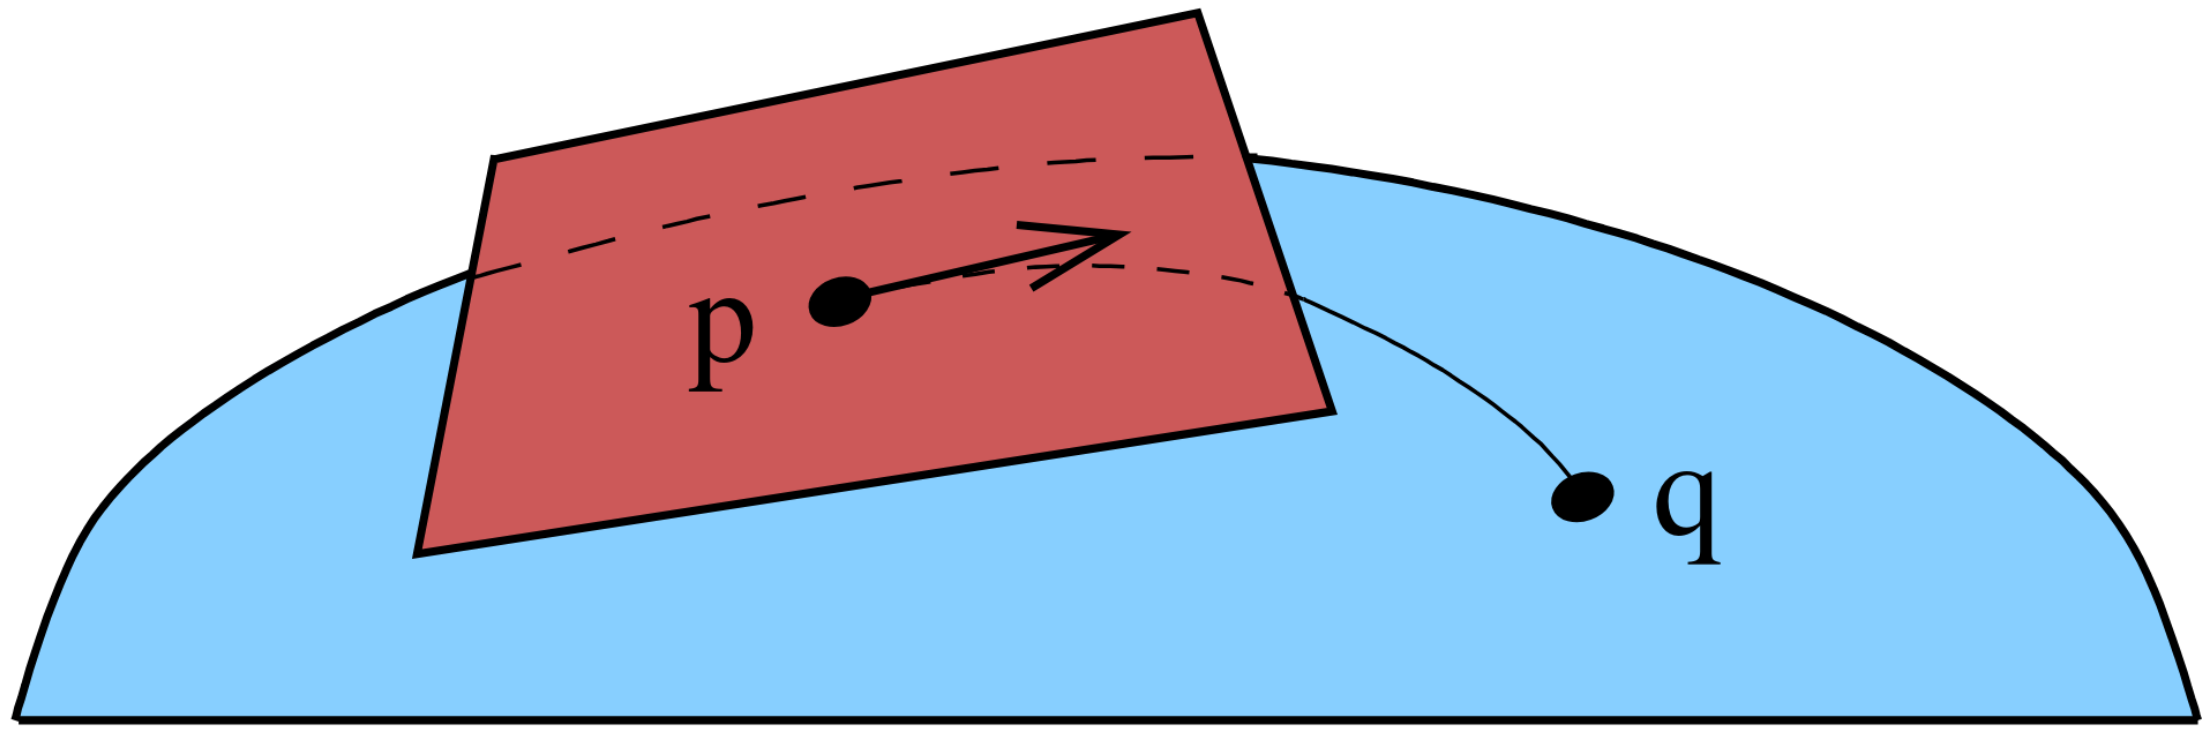
\includegraphics[width = 0.70 \textwidth]{exp-map.png}
  \caption{Visualization of the exponential map.}
  \label{exp-map}
\end{figure}

A simple way to construct normal coordinates is the following: given a tangent vector $ X_p \in T_p \mathcal{M} $, there is a unique affinely parametrized geodesic through $ p $ with tangent vector $ X_p $ at $ p $; then, any point $ q $ in the neighbourhood of $ p $ is labelled by the coordinates of the geodesic that takes from $ p $ to $ q $ a fixed amount of time.\\
Analytically, introducing a coordinate system (not necessarily normal) $ \tilde{x}^\mu $ in the neighbourhood of $ p $, an affinely parametrized geodesic solves Eq. \ref{eq:3.54}, with initial conditions $ \frac{\pa \tilde{x}^\mu}{\pa \tau}\vert_{\tau = 0} = \tilde{X}_p^\mu $ and $ \tilde{x}^\mu (\tau = 0) = 0 $ that make the solution unique. The uniqueness of the solution allows to define a map $ \Exp : T_p \mathcal{M} \rightarrow \mathcal{M} $, called the \textit{exponential map}, which acts as follows: given $ X_p \in T_p \mathcal{M} $, construct the appropriate geodesic as above and follow it for a fixed affine distance, conventionally $ \tau = 1 $, to get a new point $ q \in \mathcal{M} $. See Fig. \ref{exp-map} for visual aid. Obviously, there may be points which cannot be reached from $ p $ by geodesics, or there may be tangent vectors $ X_p $ for which $ \Exp $ is ill-defined: in General Relativity, this occurs when spacetime has singularities, but these are not relevant issues.\\
Pick a basis $ \{e_\mu\} $ of $ T_p \mathcal{M} $. Then $ \Exp : T_p \mathcal{M} \ni X^\mu e_\mu \mapsto q \in \mathcal{M} $, thus it is possible to assign coordinates in the neighbourhood of $ p $ such that $ x^\mu(q) = X^\mu $: these are the normal coordinates. To show this, note that if $ \{e_\mu\} $ is orthonormal, then the geodesics will point in orthogonal directions, ensuring that $ g_{\mu \nu}(p) = \delta_{\mu \nu} $. Now, fix a point $ q $ associated to a given tangent vector $ X_p \in T_p \mathcal{M} $: this means that $ q $ is at distance $ \tau = 1 $ from $ p $ along the given geodesic. Note that the geodesic equation is homogeneous in $ \tau $, thus in general $ \Exp : \tau X_p \mapsto x^\mu(\tau) = \tau X^\mu $, which means that geodesics take a simple form in these coordinates:
\begin{equation*}
  x^\mu (\tau) = \tau X^\mu
\end{equation*}
Being these geodesics, they must solve Eq. \ref{eq:3.54}, that is:
\begin{equation*}
  \Gamma^\mu_{\nu \rho}(x(\tau)) X^\nu X^\rho = 0
\end{equation*}
which holds at any point along the geodesic, i.e. at any $ \tau \in \R^+ $. At most points $ x(\tau) $, this equation only holds for those choices of $ X^\mu $ tangent to the geodesics. However, at $ x(0) = 0 $, i.e. at $ p $, it must hold for any tangent vector: this means that $ \Gamma^\mu_{(\nu \rho)}(p) = 0 $ which, for a torsion-free connection, ensures that $ \Gamma^\mu_{\nu \rho}(p) = 0 $. But vanishing Christoffel symbols imply a vanishing first derivative of the metric: for the Levi-Civita connection $ 2g_{\mu \sigma} \Gamma^\sigma_{\nu \rho} = g_{\mu \nu, \rho} + g_{\mu \rho, \nu} - g_{\nu \rho, \mu} $, thus symmetrizing $ (\mu \nu) $ cancels the last two terms, leaving an identity that, evaluated at $ p $, gives $ g_{\mu \nu, \rho}(p) = 0 $. Hence, these are indeed normal coordinates.

\subsubsection{Equivalence principle}

Normal coordinates are conceptually important in General Relativity: an observer at point $ p $ who parametrizes their immediate surroundings using coordinates constructed by geodesics will experience a locally flat metric. This is precisely Einstein's equivalence principle: any free-falling observer, performing local experiments, will not experience a gravitational field. The formal definition of free-falling observer is an observer which follows geodesics, while the local lack of gravitational field means $ g_{\mu \mu}(p) = \eta_{\mu \nu} $. In this context, normal coordinates are called \textit{local inertial frame}.\\
To understand what $ \virgolette{local} $ means, note that there is a way to distinguish whether a gravitational field is present at $ p $: a non-vanishing Riemann tensor. This depends on the second derivatives of the metric, which in general will be non-vanishing. However, to measure the effects of the Riemann tensor, one needs to compare the results of experiments at $ p $ and at a nearby point $ q $: this is a non-local observation.

\subsection{Curvature and torsion}

\begin{figure}[!b]
  \centering
  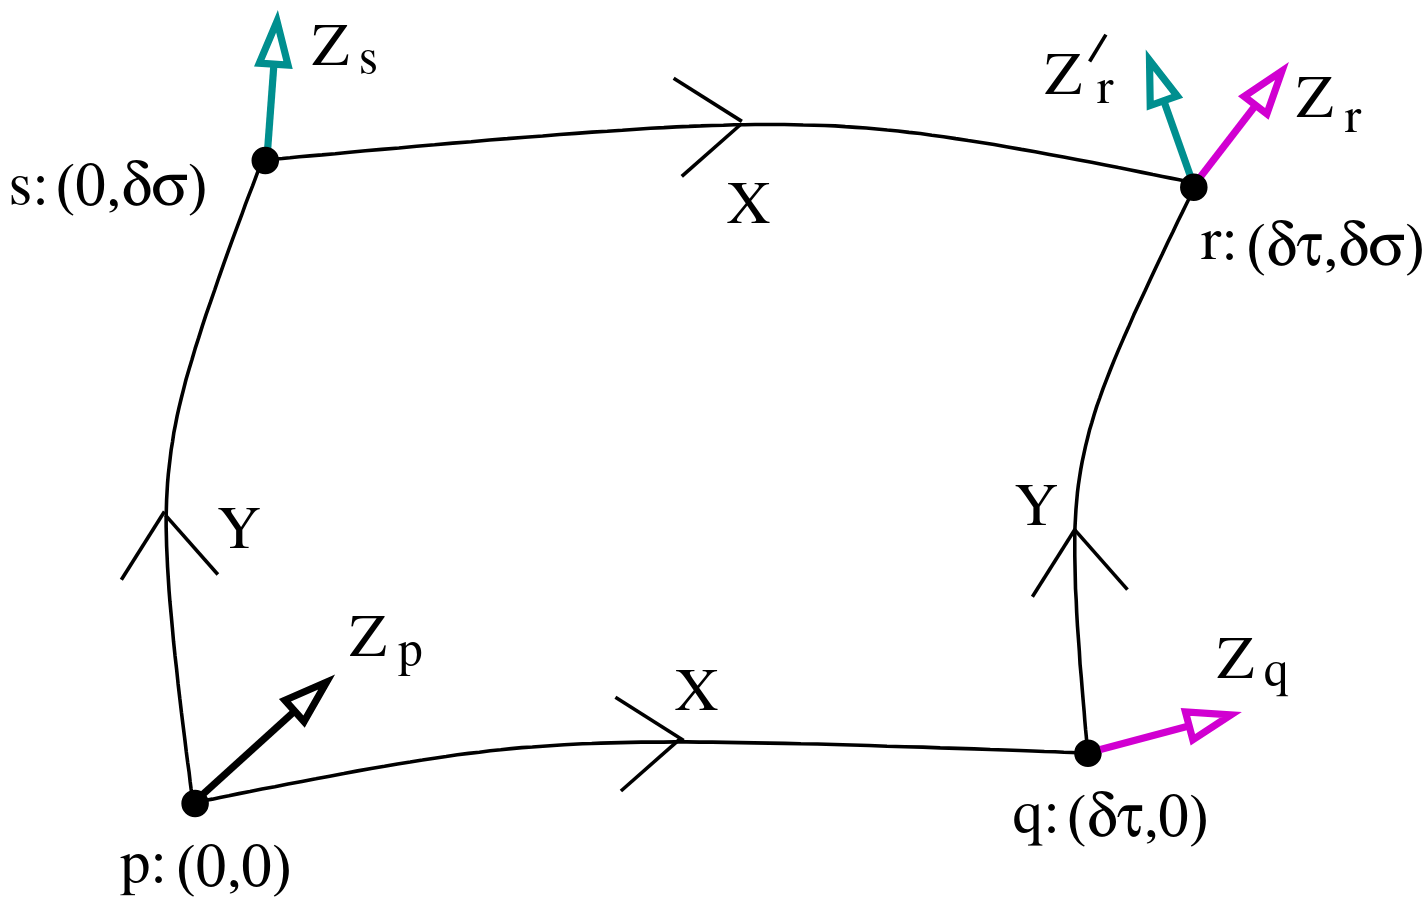
\includegraphics[width = 0.70 \textwidth]{parall-tr.png}
  \caption{Parallel transport along different paths.}
  \label{par-tr}
\end{figure}

With reference to Fig. \ref{par-tr}, consider a tangent vector $ Z_p \in T_p \mathcal{M} $ and two vector fields $ X,Y \in \xm : [X,Y] = 0 $, i.e. they are linearly independent. Construct two curved $ \gamma, \gamma' $ as in figure, both leading to a point $ r \in \mathcal{M} $ which, for simplicity, is close to $ p $. It is possible to impose normal coordinates centered at $ p $ such that $ x^\mu = (\tau, \sigma, \dots) $, so that $ X = \frac{\pa}{\pa \tau} $ and $ Y = \frac{\pa}{\pa \sigma} $: then $ x^\mu(p) = (0,0,0, \dots) $, $ X^\mu(q) = (\delta \tau, 0, 0, \dots) $, $ x^\mu(s) = (0, \delta \sigma, 0, \dots) $ and $ x^\mu(r) = (\delta \tau, \delta \sigma, 0, \dots)$, with $ \delta \tau, \delta \sigma $ small.\\
First, parallel transport $ Z_p $ along $ X $ to $ Z_q $, so that $ Z^\mu $ solves:
\begin{equation*}
  \frac{dZ^\mu}{d\tau} + X^\nu \Gamma^\mu_{\nu \rho} Z^\rho = 0
\end{equation*}
In normal coordinates $ \Gamma^\mu_{\nu \rho}(p) = 0 $, thus $ \frac{dZ^\mu}{d\tau}\big\vert_{\tau = 0} = 0 $ and the Taylor expansion is:
\begin{equation*}
  \begin{split}
    Z_q^\mu
    &= Z_p^\mu + \frac{\delta \tau^2}{2} \frac{d^2 Z^\mu}{d\tau^2}\bigg\vert_{\tau = 0} + o(\delta\tau^3) \\
    &= Z_p^\mu - \frac{\delta\tau^2}{s} \left[ X^\nu Z^\rho \frac{d\Gamma^\mu_{\nu \rho}}{d\tau} + \frac{dX^\nu}{d\tau} Z^\rho \Gamma^\mu_{\nu \rho} + X^\nu \frac{dZ^\rho}{d\tau} \Gamma^\mu_{\nu \rho} \right]_{\tau = 0} + o(\delta\tau^3) \\
    &= Z_p^\mu - \frac{\delta\tau^2}{2} X^\nu Z^\rho \frac{d\Gamma^\mu_{\nu \rho}}{d\tau}\bigg\vert_{\tau = 0} + o(\delta\tau^3) = Z_p^\mu - \frac{\delta\tau^2}{2} \left[ X^\nu X^\sigma Z^\rho \Gamma^\mu_{\nu \rho , \sigma} \right]_p + o(\delta\tau^3)
  \end{split}
\end{equation*}
where $ \frac{d}{d\tau} = X^\sigma \pa_\sigma $. Now, $ Z_q $ needs to be parallely transported along $ Y $ to $ Z_r $, but this time $ \frac{dZ^\mu}{d\sigma}\big\vert_{\sigma = 0} $ doesn't vanish, in general. From the parallel transport equation:
\begin{equation*}
  \frac{dZ^\mu}{d\sigma}\bigg\vert_{\sigma = 0} = - \left[ Y^\nu Z^\rho \Gamma^\mu_{\nu \rho} \right]_q = - \left[ Y^\nu Z^\rho X^\sigma \Gamma^\mu_{\nu \rho , \sigma} \right]_p \delta \tau + o(\delta\tau^2)
\end{equation*}
The expansions of $ Y^\nu $ and $ Z^\rho $ at leading order multiply $ \Gamma^\mu_{\nu \rho}(p) = 0 $, thus only contribute to higher order terms. Next order in $ \delta \sigma $:
\begin{equation*}
  \frac{d^2 Z^\mu}{d\sigma^2}\bigg\vert_{\sigma = 0} = - \left[ \left( \frac{dY^\nu}{d\sigma} Z^\rho + Y^\nu \frac{dZ^\rho}{d\sigma} \right) \Gamma^\mu_{\nu \rho} + Y^\nu Z^\rho \frac{d\Gamma^\mu_{\nu \rho}}{d\sigma} \right]_q = - \left[ Y^\nu Y^\sigma Z^\rho \Gamma^\mu_{\nu \rho , \sigma} \right]_p + o(\delta\tau)
\end{equation*}
The complete expansion thus is:
\begin{equation*}
  \begin{split}
    Z_r^\mu
    &= Z_q^\mu - \left[ Y^\nu Z^\rho X^\sigma \Gamma^\mu_{\nu \rho , \sigma} \right]_p \delta\tau \delta\sigma - \frac{1}{2} \left[ Y^\nu Y^\sigma Z^\rho \Gamma^\mu_{\nu \rho , \sigma} \right]_p \delta\sigma^2 + o(\delta^3) \\
    &= Z_p^\mu - \frac{1}{2} \Gamma^\mu_{\nu \rho , \sigma}(p) \left[ X^\nu X^\sigma Z^\rho \delta\tau^2 + 2 Y^\nu Z^\rho X^\sigma \delta\tau \delta\sigma + Y^\nu Y^\sigma Z^\rho \delta\sigma^2 \right] + o(\delta^3)
  \end{split}
\end{equation*}
Parallel transport along $ \gamma' $ leads to a similar expression (exchange of $ X $ and $ Y $):
\begin{equation*}
  {Z'_r}^\mu = Z_p^\mu - \frac{1}{2} \Gamma^\mu_{\nu \rho , \sigma}(p) \left[ Y^\nu Y^\sigma Z^\rho \delta\sigma^2 + 2 X^\nu Z^\rho Y^\sigma \delta\sigma \delta\tau + X^\nu X^\sigma Z^\rho \delta\tau^2 \right] + o(\delta^3)
\end{equation*}
The difference between the parallely transported tangent vectors to leading order is:
\begin{equation*}
  \Delta Z_r^\mu = Z_r^\mu - {Z'_r}^\mu = - \left[ \Gamma^\mu_{\nu \rho , \sigma} - \Gamma^\mu_{\sigma \rho , \nu} \right]_p \left[ Y^\nu Z^\rho X^\sigma \right]_p \delta\tau \delta\sigma + o(\delta^3)
\end{equation*}
Recalling that $ \Gamma^\mu_{\nu \rho}(p) = 0 $, it is possible to write:
\begin{equation}
  \Delta Z_r^\mu = - \left[ \tensor{R}{^\mu_{\rho \sigma \nu}} Y^\nu Z^\rho X^\sigma \right]_p \delta\sigma \delta\tau + o(\delta^3)
  \label{eq:3.55}
\end{equation}
It would be possible to evaluate the expression at $ r $ too, as it would differ only by higher order terms. Although the calculation was carried in a particular choice of coordinates, Eq. \ref{eq:3.55} is a tensor relation, therefore it must hold in all coordinate systems: the Riemann tensor thus determines the path dependence of parallel transport.

\subsubsection{Torsion}

\begin{figure}
  \centering
  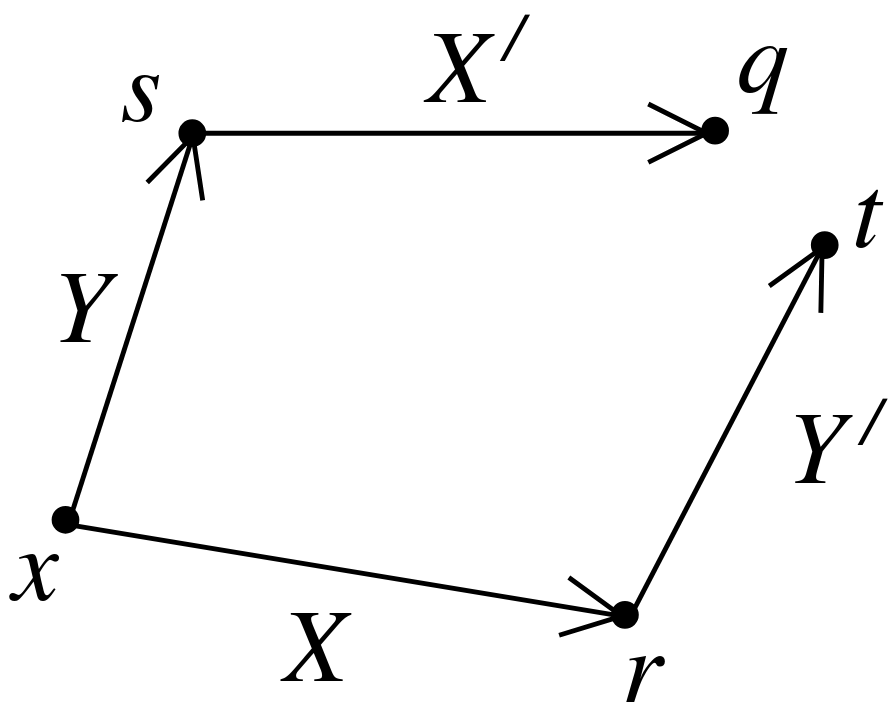
\includegraphics[width = 0.50 \textwidth]{torsion.png}
  \caption{Visualization of torsion.}
  \label{torsion}
\end{figure}

Consider two tangent vectors $ X_p,Y_p \in T_p \mathcal{M} $ and a coordinate system $ x^\mu $ such that $ X_p = X^\mu \pa_\mu $ and $ Y_p = Y^\mu \pa_\mu $. If $ p : x^\mu $, as in Fig. \ref{torsion} construct $ r,s \in \mathcal{M} $ such that $ r : x^\mu + \varepsilon X^\mu $ and $ s : x^\mu + \varepsilon Y^\mu $, with $ \varepsilon $ an infinitesimal parameter. Now, parallel transport $ X_p \in T_p \mathcal{M} $ along the direction of $ Y_p $ to $ X'_s \in T_s \mathcal{M} $ and $ Y_p \in T_p \mathcal{M} $ along $ X_p $ to $ Y'_r \in T_r \mathcal{M} $; their components will be:
\begin{equation*}
  X'_s = \left( X^\mu - \varepsilon \Gamma^\mu_{\nu \rho} Y^\nu X^\rho \right)
  \qquad \qquad
  Y'_r = \left( Y^\mu - \varepsilon \Gamma^\mu_{\nu \rho} X^\nu Y^\rho \right)
\end{equation*}
Repeating this process, starting from point $ s $ and moving along the direction of $ X'_s $, a new point $ q \in \mathcal{M} $ is determined, with coordinates:
\begin{equation*}
  q : x^\mu + \varepsilon \left( X^\mu + Y^\mu \right) - \varepsilon^2 \Gamma^\mu_{\nu \rho} Y^\nu X^\rho
\end{equation*}
Analogously, starting at point $ r $ and moving along the direction of $ Y'_r $, a new point $ t \in \mathcal{M} $ is determined, with coordinates:
\begin{equation*}
  t : x^\mu + \varepsilon \left( X^\mu + Y^\mu \right) - \varepsilon^2 \Gamma^\mu_{\nu \rho} X^\nu Y^\rho
\end{equation*}
If the connection is torsion-free, then $ q \equiv t $. On the other hand, if $ T^\mu_{\nu \rho} \neq 0 $, the parallelogram fails to close, as in Fig. \ref{torsion}.

\subsection{Geodesic deviation}

\begin{definition}
  Given a one-parameter family of geodesics $ \{x^\mu(\tau;s)\}_{s \in \R} $ on a manifold $ \mathcal{M} $, the tangent vector field and the \textit{deviation vector} field are defined as:
  \begin{equation}
    X^\mu \defeq \frac{\pa x^\mu}{\pa \tau}\bigg\vert_s
    \qquad \qquad
    S^\mu \defeq \frac{\pa x^\mu}{\pa s}\bigg\vert_\tau
    \label{eq:3.56}
  \end{equation}
\end{definition}
The meaning of these vector fields is evident: the tangent vector field fixes a particular geodesics (i.e. a particular $ s $) and assigns at each point of the geodesic its tangent vector, while the deviation vector field fixes a particular value of the affine parameter $ \tau $ and assigns at each point with this value a vector which takes to a nearby geodesic (at the same $ \tau $).

\begin{figure}
  \centering
  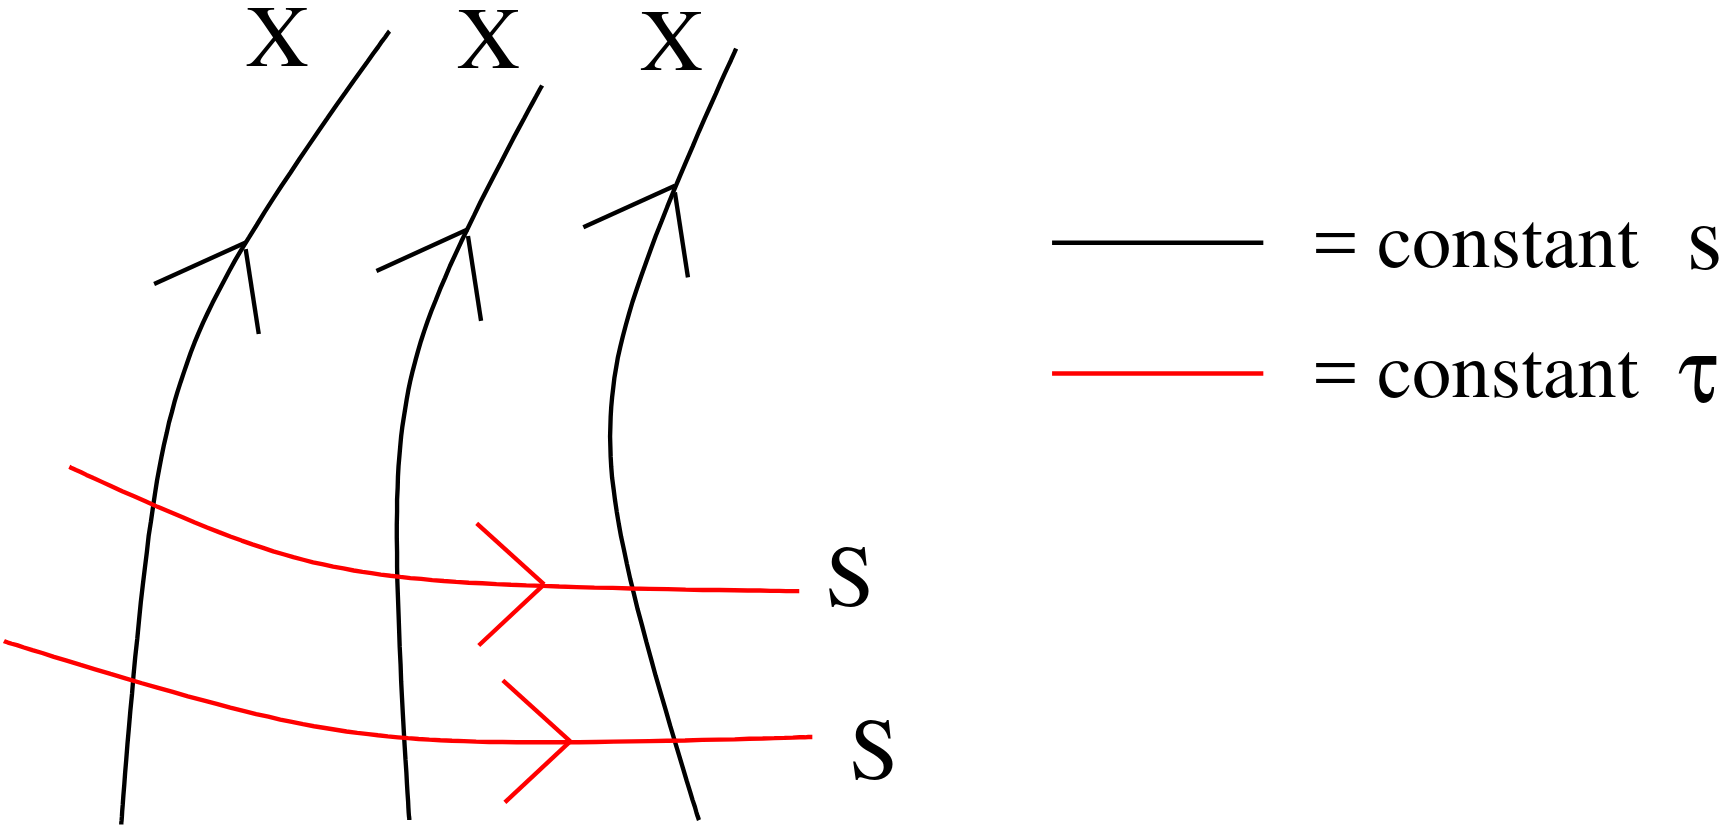
\includegraphics[width = 0.70 \textwidth]{geo-dev.png}
  \caption{A one-parameter family of geodesics generated by $ X $.}
  \label{geo-dev}
\end{figure}

The family of geodesics sweeps a surface embedded in the manifold, so there is freedom in the choice of coordinates $ s $ and $ \tau $. In particular, it's always possible to pick them so that $ X = \frac{\pa}{\pa \tau} $ and $ S = \frac{\pa}{\pa s} $, in order for them to be linearly independent: $ [X,S] = 0 $, as in Fig. \ref{geo-dev}. Consider a torsion-free connection, so that:
\begin{equation*}
  \na_X S - \na_S X = [X,S] = 0
  \qquad \Rightarrow \qquad
  \na_X \na_X S = \na_X \na_S X = \na_S \na_X X + R(X,S) X
\end{equation*}
But $ X $ is tangent to geodesics, so from Eq. \ref{eq:3.53} $ \na_X X = 0 $ and:
\begin{equation}
  \na_X \na_X S = R(X,S) X
  \label{eq:3.57}
\end{equation}
Restricting to an integral curve $ \gamma $ of the vector field $ X $, i.e. $ X^\mu \vert_\gamma = \frac{dx^\mu}{d\tau} $, the covariant derivative along $ \gamma $ becomes:
\begin{equation*}
  \na_X\big\vert_\gamma = X^\mu\big\vert_\gamma \na_\mu = \frac{dx^\mu}{d\tau} \na_\mu \equiv \frac{D}{D\tau}
\end{equation*}
Hence, in index notation, the change of the deviation vector along the geodesic is expressed as:
\begin{equation}
  \frac{DS^\mu}{D\tau} = \tensor{R}{^\mu _{\nu \rho \sigma}} X^\rho S^\sigma X^\nu
  \label{eq:3.58}
\end{equation}
This can be interpreted as the relative acceleration of neighbouring geodesics, and it is determined by the Riemann tensor. Experimentally, such geodesic deviations are called \textit{tidal forces}.

\section{Riemann tensor}

Recall Eq. \ref{eq:3.36} for the components of the Riemann tensor $ \tensor{R}{^\sigma _{\rho \mu \nu}} $: it is manifestly anti-symmetric in its last two indices, but there are also other subtle symmetries when using the Levi-Civita connection.

\begin{proposition}
  On a metric manifold with a Levi-Civita connection:
  \begin{equation}
    R_{\sigma \rho \mu \nu} = - R_{\sigma \rho \nu \mu} = - R_{\rho \sigma \mu \nu} = R_{\mu \nu \sigma \rho}
    \label{eq:3.59}
  \end{equation}
  \begin{equation}
    R_{\sigma [\rho \mu \nu]} = 0
    \label{eq:3.60}
  \end{equation}
\end{proposition}
\begin{proof}
  Set normal coordinates centered at a point $ p $: then, $ \Gamma^\mu_{\nu \rho} = 0 $ and $ \pa_\mu g^{\lambda \sigma} = 0 $ at that point. At $ p $, the Riemann tensor can be written as:
  \begin{equation*}
    \begin{split}
      R_{\sigma \rho \mu \nu}
      &= g_{\sigma \lambda} \tensor{R}{^\lambda _{\rho \mu \nu}} = g_{\sigma \lambda} \left[ \pa_\mu \Gamma^\lambda_{\nu \rho} - \pa_\nu \Gamma^\lambda_{\mu \rho} \right] \\
      &= \frac{1}{2} \left[ \pa_\mu \left( \pa_\nu g_{\sigma \rho} + \pa_\rho g_{\nu \sigma} - \pa_\sigma g_{\nu \rho} \right) - \pa_\nu \left( \pa_\mu g_{\sigma \rho} + \pa_\rho g_{\mu \sigma} - \pa_\sigma g_{\mu \rho} \right) \right] \\
      &= \frac{1}{2} \left[ \pa_\mu \pa_\rho g_{\nu \sigma} - \pa_\mu \pa_\sigma g_{\nu \rho} - \pa_\nu \pa_\rho g_{\mu \sigma} + \pa_\nu \pa_\sigma g_{\mu \rho} \right]
    \end{split}
  \end{equation*}
  The symmetries are then manifest, and being these tensor equations they are valid in all coordinate systems.
\end{proof}

An important computation tool is the \textit{Bianchi identity}.

\begin{theorem}[Bianchi]
  On a metric manifold with a Levi-Civita connection:
  \begin{equation}
    \na_{[\lambda} R_{\sigma \rho] \mu \nu} = 0
    \qquad \Leftrightarrow \qquad
    \tensor{R}{^\sigma_{\rho [\mu \nu ; \lambda]}} = 0
    \label{eq:3.61}
  \end{equation}
\end{theorem}
\begin{proof}
  The two equations are equivalent, so the proof is of the first one. In normal coordinates $ \na_\mu = \pa_\mu $ at $ p $, so schematically: $ R = \pa \Gamma + \Gamma \Gamma $, thus $ \na R = \pa R = \pa^2 \Gamma + \Gamma \pa \Gamma = \pa^2 \Gamma $. Explicitly:
  \begin{equation*}
    \pa_\lambda R_{\sigma \rho \mu \nu} = \frac{1}{2} \pa_\lambda \left[ \pa_\mu \pa_\rho g_{\nu \sigma} - \pa_\mu \pa_\sigma g_{\nu \rho} - \pa_\nu \pa_\rho g_{\mu \sigma} + \pa_\nu \pa_\sigma g_{\mu \rho} \right]
  \end{equation*}
  Anti-symmetrizing the appropriate indices yields the result.
\end{proof}

Note that Eq. \ref{eq:3.60}-\ref{eq:3.61} do not require that the connection is a Levi-Civita connection, but are valid for general torsion-free connections.

\subsection{Ricci and Einstein tensors}

\begin{definition}
  On a metric manifold, the \textit{Ricci tensor} is defined as:
  \begin{equation}
    R_{\mu \nu} \defeq \tensor{R}{^\rho _{\mu \rho \nu}}
    \label{eq:3.62}
  \end{equation}
  The \textit{Ricci scalar} is defined as:
  \begin{equation}
    R \defeq g^{\mu \nu} R_{\mu \nu}
    \label{eq:3.63}
  \end{equation}
\end{definition}

\begin{proposition}
  On a metric manifold with a Levi-Civita connection:
  \begin{equation}
    R_{\mu \nu} = R_{\nu \mu}
    \label{eq:3.64}
  \end{equation}
\end{proposition}
\begin{proof}
  Using Eq. \ref{eq:3.59}: $ R_{\mu \nu} = g^{\sigma \rho} R_{\sigma \mu \rho \nu} = g^{\rho \sigma} R_{\rho \nu \sigma \mu} = R_{\nu \mu} $.
\end{proof}

\begin{proposition}
  On a metric manifold:
  \begin{equation}
    \na^\mu R_{\mu \nu} = \frac{1}{2} \na_\nu R
    \label{eq:3.65}
  \end{equation}
\end{proposition}
\begin{proof}
  Writing explicitly Bianchi identity:
  \begin{equation*}
    \na_\lambda R_{\sigma \rho \mu \nu} + \na_\sigma R_{\rho \lambda \mu \nu} + \na_\rho R_{\lambda \sigma \mu \nu} = 0
  \end{equation*}
  Contracting with $ g^{\mu \lambda} g^{\rho \nu} $:
  \begin{equation*}
    \na^\mu R_{\mu \sigma} - \na_\sigma R + \na^\nu R_{\nu \sigma} = 0
  \end{equation*}
  which yields the thesis.
\end{proof}

\begin{definition}
  On a metric manifold, the \textit{Einstein tensor} is defined as:
  \begin{equation}
    G_{\mu \nu} \defeq R_{\mu \nu} - \frac{1}{2} R g_{\mu \nu}
    \label{eq:3.66}
  \end{equation}
\end{definition}

\begin{proposition}
  On a metric manifold, the Einstein tensor is covariantly constant:
  \begin{equation}
    \na^\mu G_{\mu \nu} = 0
    \label{eq:3.67}
  \end{equation}
\end{proposition}
\begin{proof}
  Trivial from Eq. \ref{eq:3.65}.
\end{proof}

\subsection{Connection and curvature forms}

This section is based on a Lorentzian manifold, but the discussion is equivalent on a Riemannian one: it's enough to swap $ \eta_{ab} $ with $ \delta_{ab} $ as the flat metric.

\subsubsection{Vielbeins}

Although typically calculations are carried on a coordinate basis $ \{e_\mu\} = \{\pa_\mu\} $, there are possible basis without such an interpretation. For example, a linear combination of a coordinate basis won't in general be a coordinate basis itself:
\begin{equation}
  \hat{e}_a = \tensor{e}{_a^\mu} \pa_\mu
  \label{eq:3.68}
\end{equation}
A particularly useful non-coordinate basis is one such that:
\begin{equation}
  g(\hat{e}_a, \hat{e}_b) = g_{\mu \nu} \tensor{e}{_a^\mu} \tensor{e}{_b^\nu} = \eta_{ab}
  \label{eq:3.69}
\end{equation}
The components $ \tensor{e}{_a^\mu} $ are called \textit{vielbeins} or \textit{tetrads}. In this non-coordinate system, the manifold looks flat (or, at least, its patch covered by the given chart). In the following computations, greek indices are raised/lowered by the metric $ g_{\mu \nu} $, while latin indices by the metric $ \eta_{ab} $.\\
The vielbeins aren't unique, for given a set of vielbeins $ \tensor{e}{_a^\mu} $ it is always possible to find a new one:
\begin{equation}
  \tensor{\tilde{e}}{_a^\mu} = \tensor{e}{_b^\mu} \tensor{(\Lambda^{-1})}{^b_a}
  \label{eq:3.70}
\end{equation}
The transformation matrix must satisfy the condition imposed by Eq. \ref{eq:3.69}, i.e.:
\begin{equation}
  \tensor{\Lambda}{_a^c} \tensor{\Lambda}{_b^d} \eta_{cd} = \eta_{ab}
  \label{eq:3.71}
\end{equation}
These are \textit{local Lorentz transformations}, because the condition is that of Lorentz transformation, but $ \Lambda $ is now allowed to vary over the manifold. The dual basis of one-forms $ \{\hat{\theta}^a\} $ is defined by $ \hat{\theta}^a(\hat{e}_b) = \delta^a_b $. The relation to the coordinate basis is:
\begin{equation}
  \hat{\theta}^a = \tensor{e}{^a_\mu} dx^\mu
  \label{eq:3.72}
\end{equation}
where the coefficients satisfy:
\begin{equation}
  \tensor{e}{^a_\mu} \tensor{e}{_b^\mu} = \delta^a_b
  \label{eq:3.73}
\end{equation}
\begin{equation}
  \tensor{e}{^a_\mu} \tensor{e}{_a^\nu} = \delta_\mu^\nu
  \label{eq:3.74}
\end{equation}
The metric is a tensor, so $ g = g_{\mu \nu} dx^\mu \otimes dx^\nu = \eta_{ab} \hat{\theta}^a \otimes \hat{\theta}^b $, thus it is related to the vielbeins by:
\begin{equation}
  g_{\mu \nu} = \tensor{e}{^a_\mu} \tensor{e}{^b_\nu} \eta_{ab}
  \label{eq:3.75}
\end{equation}

\subsubsection{Connection 1-form}

On a non-coordinate basis $ \{\hat{e}_a\} $, connection components are computed in the usual way:
\begin{equation}
  \na_{\hat{e}_c} \hat{e}_b = \Gamma^a_{cb} \hat{e}_a
  \label{eq:3.76}
\end{equation}
However, these are not the same components $ \Gamma^\mu_{\nu \rho} $ as in a coordinate basis.

\begin{definition}
  On a metric manifold with vielbeins, the \textit{connection 1-form} is defined as:
  \begin{equation}
    \tensor{\omega}{^a_b} \defeq \Gamma^a_{cb} \hat{\theta}^c
    \label{eq:3.77}
  \end{equation}
\end{definition}

Note that these are really $ n^2 $ 1-forms, according to values of $ a,b = 1, \dots, n \equiv \dim_{\R} \mathcal{M} $. This is also known as the \textit{spin connection}, due to its relationship to spinors in curved spacetime.

\begin{proposition}
  Given a local Lorentzian transformation $ \Lambda $:
  \begin{equation}
    \tensor{\tilde{\omega}}{^a_b} = \tensor{\Lambda}{^a_c} \tensor{\omega}{^c_d} \tensor{(\Lambda^{-1})}{^d_b} + \tensor{\Lambda}{^a_c} \tensor{(d\Lambda^{-1})}{^c_b}
    \label{eq:3.78}
  \end{equation}
\end{proposition}

The second term reflects the second term in Prop. \ref{gamma-non-tens}, which involves the derivative of the coordinate transformation. Important results for connection 1-forms is the \textit{Cartan structure equation}.

\begin{theorem}[Cartan]
  On a metric manifold with a torsion-free connection:
  \begin{equation}
    d\hat{\theta}^a + \tensor{\omega}{^a_b} \wedge \hat{\theta}^b = 0
    \label{eq:3.79}
  \end{equation}
\end{theorem}
\begin{proof}
  From Eq. \ref{eq:3.76} $ \Gamma^a_{cb} = \tensor{e}{^a_\rho} \tensor{e}{_c^\mu} \na_\mu \tensor{e}{_b^\rho} $, thus, remembering $ \Gamma^\rho_{[\mu \nu]} = 0 $ (torsion-free):
  \begin{equation*}
    \begin{split}
      \tensor{\omega}{^a_b} \wedge \hat{\theta}^b
      &= \Gamma^a_{cb} \left( \tensor{e}{^c_\mu} dx^\mu \right) \wedge \left( \tensor{e}{^b_\nu} dx^\nu \right) \\
      &= \tensor{e}{^a_\rho} \tensor{e}{_c^\mu} \left( \pa_\mu \tensor{e}{_b^\rho} + \tensor{e}{_b^\nu} \Gamma^\rho_{\mu \nu} \right) \left( \tensor{e}{^c_\mu} dx^\mu \right) \wedge \left( \tensor{e}{^b_\nu} dx^\nu \right) \\
      &= \tensor{e}{^a_\rho} \underbrace{\tensor{e}{_c^\lambda} \tensor{e}{^c_\mu}}_{\delta_\mu^\lambda} \tensor{e}{^b_\nu} \left( \pa_\lambda \tensor{e}{_b^\rho} + \tensor{e}{_b^\sigma} \Gamma^\rho_{\lambda \sigma} \right) dx^\mu \wedge dx^\nu = \tensor{e}{^a_\rho} \tensor{e}{^b_\nu} \pa_\mu \tensor{e}{_b^\rho} dx^\mu \wedge dx^\nu
    \end{split}
  \end{equation*}
  But $ \tensor{e}{^b_\nu} \tensor{e}{_b^\rho} = \delta_\nu^\rho $, so $ \tensor{e}{^b_\nu} \pa_\mu \tensor{e}{_b^\rho} = - \tensor{e}{_b^\rho} \pa_\mu \tensor{e}{^n_\nu} $, hence:
  \begin{equation*}
    \tensor{\omega}{^a_b} \wedge \hat{\theta}^b = - \tensor{e}{^a_\rho} \tensor{e}{_b^\rho} \pa_\mu \tensor{e}{^b_\nu} dx^\mu \wedge dx^\nu = - \pa_\mu \tensor{e}{^a_\nu} dx^\mu \wedge dx^\nu = -d\hat{\theta}^a
  \end{equation*}
\end{proof}

For a Levi-Civita connection, a stronger result holds.

\begin{proposition}
  On a metric manifold with a Levi-Civita connection:
  \begin{equation}
    \omega_{ab} = -\omega_{ba}
    \label{eq:3.80}
  \end{equation}
\end{proposition}
\begin{proof}
  Being the Levi-Civita connection compatible with the metric:
  \begin{equation*}
    \begin{split}
      \Gamma_{abc}
      &= \eta_{ad} \tensor{e}{^d_\rho} \tensor{e}{_b^\mu} \na_\mu \tensor{e}{_c^\rho} = -\eta_{ad} \tensor{e}{_c^\rho} \tensor{e}{_b^\mu} \na_\mu \tensor{e}{^d_\rho} = -\eta_{cf} \tensor{e}{^f_\sigma} \tensor{e}{_b^\mu} \na_\mu (\eta_{ad} g^{\rho \sigma} \tensor{e}{^d_\rho}) \\
      &= -\eta_{cf} \tensor{e}{^f_\rho} \tensor{e}{_b^\mu} \na_\mu \tensor{e}{_a^\rho} = -\Gamma_{cba}
    \end{split}
  \end{equation*}
  From Eq. \ref{eq:3.77} $ \omega_{ab} = \Gamma_{acb} \hat{\theta}^c $, thus completing the proof.
\end{proof}

Eq. \ref{eq:3.79}-\ref{eq:3.80} allow to quickly compute the spin connection, as they uniquely define it. Indeed, $ \omega_{ab} $ being anti-symmetric means that there are $ \frac{1}{2} n (n-1) $ independent 1-forms, i.e. $ \frac{1}{2} n^2 (n-1) $ independent components. The Cartan structure equation relates two 2-forms, each with $ \frac{1}{2} n (n-1) $ independent components, thus posing $ \frac{1}{2} n^2 (n-1) $ constraints (as there are $ n $ equations) and uniquely fixing the spin connection.

\subsubsection{Curvature 2-form}

Recall Eq. \ref{eq:3.59}, which holds for Levi-Civita connections. Computing the Riemann tensor in the non-coordinate basis $ \tensor{R}{^a_{bcd}} = R(\hat{\theta}^a, \hat{e}_b, \hat{e}_c, \hat{e}_d) $, the anti-symmetry of the last two indices persists: $ \tensor{R}{^a_{bcd}} = -\tensor{R}{^a_{bdc}} $.

\begin{definition}
  On a metric manifold with a Levi-Civita connection, the \textit{curvature 2-form} is defined as:
  \begin{equation}
    \tensor{\mathcal{R}}{^a_b} \defeq \frac{1}{2} \tensor{R}{^a_{bcd}} \hat{\theta}^c \wedge \hat{\theta}^d
    \label{eq:3.81}
  \end{equation}
\end{definition}

Again, these are really $ n^2 $ 2-forms. A second \textit{Cartan structure relation} holds.

\begin{theorem}[Cartan]
  On a metric manifold with a Levi-Civita connection:
  \begin{equation}
    \tensor{\mathcal{R}}{^a_b} = \tensor{d\omega}{^a_b} + \tensor{\omega}{^a_c} \wedge \tensor{\omega}{^c_b}
    \label{eq:3.82}
  \end{equation}
\end{theorem}

Connection and curvature forms make computing the Riemann tensor less tedious, as exterior derivatives take significant less effort than covariant derivatives.










